\documentclass[10pt,a4paper,final]{report}
\usepackage{amsmath}
\usepackage{amsfonts}
\usepackage{listings}
\usepackage{graphicx} % Required for including images
\usepackage[font=small,labelfont=bf]{caption} % Required for specifying captions to tables and figures
\usepackage{hyperref}
\usepackage[utf8]{inputenc}
\usepackage[spanish]{babel}
\usepackage{amsthm}
\usepackage{graphicx}
\newtheorem{theorem}{Teorema}
\newtheorem{lemma}{Lema}
\newtheorem{definition}{Definición}
\newtheorem{proposition}{Proposición}
\newtheorem{observation}{Observación}
\newtheorem{corollary}{Corolario}
\newtheorem{example}{Ejemplo}

\newtheorem{caution}{¡Cuidado!}


\def\Q{\mathbb{Q}}
\def\R{\mathbb{R}}
\def\C{\mathbb{C}}
\def\I{[a,b]} 

\begin{document}


\section{Punto flotante y redondeo}
{
	Sea $x=0,a_1 a_2...a_m... 10^l$. Es decir, x está en el rango de la máquina (podría no estarlo y en ese caso no podríamos aproximarlo bien).
	
Hay dos formas de aproximar a $x$. Una es por truncamiento y la otra por redondeo.

Recordemos que a nosotros nos interesa más que nada medir el error relativo de las cuentas que hacemos: si el número que trabajamos es muy pequeño los errores pequeños nos van a importar: no es lo mismo pifiarle 0.1 cm a la distancia de la Tierra a la Luna que a la medida de una pieza de laboratorio.

¿Cómo es el error absoluto, y el relativo en truncamiento y redondeo?

\begin{itemize}
	\item Truncamiento: $|x-x^*| = 0,0...0a_{m+1}a_{m+2}$...$ 10^l \geq 10^{l-m}$ porque los $a_j$ podrían ser todos 9.
	\item Redondeo: $|x-x^*| \geq 0,0$...$05$ . $ 10^l = \frac{1}{2} 10^{l-m}$. Esta cuenta también se puede hacer contando la cantidad de números de máquina entre $10^{l-1}$ y $10^{l}$, que están uniformemente distribuidos. Son $9\cdot 10^{m-1}$. La distancia entre $x$ y $x^*$ va a ser menor o igual a la mitad de la distancia entre dos números de máquina en $[10^{l-1}, 10^{l}]$ porque siempre se toma el más cercano, es decir, $\frac{9\ 10^{l-1}}{2\cdot 9\cdot 10^{m-1}} = \frac{1}{2} 10^{l-m}$, como queríamos ver.
\end{itemize}

%TODO hablar de las cancelaciones catastróficas y cómo se arreglan

\subsection{$\varepsilon$ de la máquina}

\subsection{Problemas al redondear y cómo evitarlos}

\begin{itemize}
	\item Sumar números de órdenes muy distintos $x >> y$ lleva a que al redondear $x+y$ podamos llegar a obtener $x$ o parecido, como si no hubiéramos sumado $y$. Un ejemplo particular es hacer $1+\varepsilon'$, o también $x + |x| \varepsilon'$, con $\varepsilon' < \varepsilon$. Si tenemos en cuenta esto, se ve que al sumar una lista de números conviene sumarlos de menor a menor. Es más, tal vez convendría cada vez que se suman dos números de la lista, reemplazarlos por el número sumado y volver a ordenar de menor a mayor la nueva lista (porque el resultado pudo haber quedado mayor que otros números). Un ejemplo artificial sería tener que sumar $\{0.01\}$ 10000 veces y el número 10. Si solo se ordena la lista de menor a mayor una vez, entonces luego de sumar los primeros 1000 números queda $1000$ y al sumarlo con $10$ estaríamos sumando números de órdenes muy distintos.
%TODO esto está escrito para el orto. Hablar más y mejor de por qué cuando dos números están cerca nos interesa que el error sea muy pequeño
	\item Cancelación catastrófica (cuando se restan números muy parecidos) Puede pasar que se pierdan dígitos significativos del resultado. Recordemos que a nosotros nos interesa medir el \textit{error relativo} así que si $x$ e $y$ están muy cerca y los restamos, al redondear podemos obtener un error que puede parecer pequeño pero al dividir por $|x-y|$ obtenemos que el error relativo es grande. Algunos ejemplos:
	\begin{itemize}
		\item Un ejemplo es hacer $y = \sqrt{x^+1}-1$ para valores de $x$ pequeños. ¡Lo que se puede hacer para salvar esto es multiplicar y dividir por el conjugado!
		\item Otro es la querida resolvente aplicada a una ecuación cuadrática. La observación que se puede hacer es que si (SPG, sin perder generalidad) $-b - \sqrt{b^2-4ac}$ es una resta de números parecidos y eso me está generando errores, puedo calcular la \textit{otra} raíz, que necesariamente no va a tener una resta de números parecidos porque hay que hacer $-b + \sqrt{b^2-4ac}$ y luego usar la fórmula $x_2 = \frac{c}{a x_1}$ para calcular la primer raíz.
		\item Triangulación de matrices a la Gauss: para triangular se multiplica la primer fila por $\frac{a_{j1}}{a_{11}}$ y se resta la fila $j$. Una vez obtenidos ceros en $a_{1j}$ para $j>1$ se procede inductivamente sobre la submatriz que queda al eliminar la primer fila y la primer columna. El problema de hacer esto es que $\frac{a_{j1}}{a_{11}}$ puede ser muy grande y al restar filas podríamos estar restando números de órdenes muy distintos (lo cuál es tan malo como sumar números de órdenes muy distintos porque se pierde la información del número pequeño). La solución a este problema es intercambiar filas, dejando como $a_{11}$ al más grande, para que $\frac{a_{j1}}{a_{11}}$ sea pequeño.
	\item A veces el problema mismo está "mal condicionado", en el sentido de que pequeños errores en los datos (al redondear, por ejemplo), producen grandes cambios en la solución. Un ejemplo de esto se da al trabajar con matrices. Veremos algunos teoremas más adelante.
	\end{itemize}
\end{itemize}

}


\section{Metodos de un paso}
%TODO agregar tildes
\begin{theorem}
    Para $n\in \mathbb{N}$ y $h=(T-t_0)/n$ consideremos el método de un paso dado por $x_{i+1}=x_i + h \Phi(t_i,x_i,h)$ con $\Phi$ una función Lipchitz en la segunda variable con constante $K$. Entonces:
    
    $$|x(T)-x_n|\leq \frac{\tau_{max}}{K} (e^{K(t-t_0)}-1)$$
\end{theorem}

\begin{proof}
    La idea es acotar $e_i$ y después acumular.
    
    $e_i := x(t_i)-x_i$ el error global hasta el paso $i$. Tenemos: \\
    
    $$x_{i+1}=x_i + h \Phi(t_i,x_i,h)$$
    $$x(t_{i+1})=x(t_i) + h \Phi(t_{i},x(t_i),h) + h \tau_i$$
    
    donde la segunda igualdad es la definición del error. \\
    
    Luego $e_{i+1} = e_i + h (\Phi(t_{i},x(t_{i}),h) - \Phi(t_i,x_i,h)) + \tau_i$.
    
    Luego $|e_{i+1}| \leq |e_i| + hK |x_i-x(t_i)| + h\tau_{max} = (1+hK) |e_i| + h\tau_{max}$
    
\begin{caution}
	¡¡No olvidarse de cambiar $\tau_i$ por $\tau_{max}$!!    
\end{caution}
    
    Si llamamos $A = 1 + hK$, podemos iterar esto.
    
    
    $$|e_0| = 0$$
    $$|e_1| \leq h\tau_{max}$$
    $$|e_2| \leq A |e_1| + h\tau_{max} \leq (A+1) h\tau_{max}$$
    $$|e_3| \leq A |e_2|+ h\tau_{max} \leq (A^2+A+1) h\tau_{max}$$
    (...)
    $$|e_n| \leq (A^{n-1}+...+A+1) h\tau_{max} = h\tau_{max} \frac{A^{n}-1}{A-1} = \frac{\tau_{max}}{K} ((1+Kh)^n-1)$$
    
    Ahora bien, $e^x-x-1\geq0$ en $x\geq0$, eso se puede ver derivando.
    Entonces $e^x \geq x+1$ y por lo tanto $e^{xn}\geq (x+1)^n$ si $x\geq0$. Tomando $x=1+Kh$, queda que la expresión de arriba es menor o igual a $\frac{\tau_{max}}{K} (e^{nKh}-1)$ y como $nH = T - t_0$, estamos.
    
\end{proof}

\begin{caution}
\begin{itemize}
	\item[]
	\item No olvidarse de que los $\tau_i$ no son todos iguales y justamente acotamos por $\tau_{max}$ (que es finito siempre porque es el máximo de finitas diferencias)
	\item No olvidarse de usar que $hN = T - t_0$
\end{itemize}
\end{caution}


\subsection*{Métodos de Runge Kutta}

La idea de estos métodos es alcanzar el mismo orden que un metodo de Taylor de orden k pero sin tener que derivar.

A modo de ejemplo, encontremos un método de RK de orden 2.

El método de Taylor de orden 2 se basa en la igualdad $x(t+h)= x(t) + h T_2(t,x(t),h) + O(h^3)$

Nosotros buscamos reemplazar $T_2$ por una $Phi_2$ en la que no haya que derivar a $f$. para eso, basta tener $T_2 - Phi_2 = O(h^2)$


$x(t+h) = x(t) + hf(t,x) + \frac{h^2}{2} [f_t(t,x) + f_x(t,x) f_t(t,x)] + O(h^3)$. Tenemos $T_2(t,x,h) = f(t,x) + \frac{h}{2} [f_t(t,x) + f_x(t,x) f_t(t,x)]$

Planteo $\Phi_2(t,x) = A_1 f(t,x) + A_2 f(t + \alpha h, x + \alpha h f(t,x))$. No estoy seguro por que es natural que a un incremento de $\alpha h$ en $t$ corresponda el otro incremento en la variable $x$.

Hagamos Taylor en varias variables:

$f(t + \alpha h, x + \alpha h f(t,x)) = f(t,x) + \alpha h f_t(t,x) + \alpha h f(t,x) f_x(t,x)$. Me parece que esto esta bien hecho y que al derivar en la primer variable no hay que hacer regla de la cadena, pero no estoy seguro por que.

Tenemos $\Phi_2(t,x,h) = (A_1 + A_2) f(t,x) + A_2 \alpha h [f_t(t,x) + f(t,x) f_x(t,x)] + O(h^2)$

Para que la resta tenga orden $h^2$, todo se debe cancelar. Luego obtenemos lo deseado si pedimos:

$A_1 + A_2 = 1, A_2 \alpha = \frac{1}{2}$.

Si despejamos obtenemos: $A_2 = \frac{1}{2 \alpha}$, $A_1 = 1 - \frac{1}{2 \alpha}$.

Es decir, obtuvimos infinitas soluciones, una por cada $\alpha \neq 0$.


Eligiendo $\alpha=\frac{1}{2}$ se obtiene el llamado metodo de Euler modificado, y eligiendo $\alpha=1$ se obtiene el famosisimo método de Heun. Espero que no me tomen los nombres. Una regla mnemotécnica podria ser que el Euler modificado es el "menos distinto" :-)



\begin{proposition}
    Se dice que un método es convergente si la solucion numerica tiende a cero si h tiende a cero. En los métodos de un paso, basta que $\tau$ tienda a cero para que esto suceda. Esto se denomina consistencia del método y en los métodos de un paso consistencia y convergencia son conceptos equivalentes.
    
    Si asumimos $\Phi$ continua, se tiene que la consistencia es equivalente a que $x'(t_i) = \Phi(t_i,x(t_i),0)$. Me parece que esto se da porque entonces uno con Taylor ve que cuando h tiende a cero el método se porta igual que Euler de orden 1.
    
\end{proposition}


\begin{observation}
    Todos los métodos que conocemos son convergentes
\end{observation}


\begin{proof}
    Basta evaluar en donde corresponde.
\end{proof}




\section{Diferencias finitas}


\begin{definition}
    Se dice que un método estable si es Lipchitz con respecto a los datos iniciales, es decir, si $||u^n-v^n||_{\infty} \leq C ||u^0-v^0||_{\infty}$ con c constante fija (en particular no depende de n). Por linealidad, es lo mismo que pedir $||w^n||_{\infty} \leq C ||w^0||_{\infty}$
\end{definition}

\begin{observation}
    Basta que $||A||_\infty^n$ este acotada.
\end{observation}

TODO: me falta entender mejor que es estabilidad. En la teorica vieron una definicion alternativa. Tambien me falta ver el teorema de consistencia + estabilidad implica convergencia


\begin{definition}
	Se dice que un problema tiene condición de borde de tipo Dirichlet si la solución es cero en el borde del dominio espacial para todo valor de $t$.
\end{definition}

\begin{definition}
	Se duce que un problema es consistente si $T_j^n\to 0$ si $k\to 0, h\to 0, \forall j,n$, donde $T_j^n$ es el error de truncado...y está definido distinto en las diferentes fuentes que encontré.
	
	En la materia el error de truncado lo definieron como reemplazar en la ecuación diferencial las derivadas por las aproximaciones y ver cuánto nos alejamos de la igualdad.
\end{definition}


\section{SVD}

Ver https://blog.statsbot.co/singular-value-decomposition-tutorial-52c695315254 y tambien http://andrew.gibiansky.com/blog/mathematics/cool-linear-algebra-singular-value-decomposition/

Está mucho mejor explicado en la teórica, pero igual:

Queremos $A V = U \Sigma$


%TODO por que no anda A A^*?
%TODO hacer ejercicios de "para que sirve SVD" de la guia

Consideramos $A^* A$. Es hermitiana y semi definida positiva, así que existe base de autovectores $(v_i)$ con autovalores positivos $\sigma_1^2 \geq \sigma_2^2 \geq ... \geq \sigma_n^2 \geq 0$

Si $r = rg A$, llamo $u_i = \frac{1}{\sigma_i} A v_i \forall i \leq r$ (son los que tienen que ser)

Estos cumplirán ser ortonormales (el denominador se pone para que sean normales):

$u_i \cdot  u_j = \frac{1}{\sigma_i \sigma_j} <Av_i, Av_j> = \frac{1}{\sigma_i \sigma_j}<v_i, A^t A v_j> = <v_i, \sigma_j^2 v_j> = \frac{1}{\sigma_i \sigma_j} \delta_{ij} \sigma_j^2$\\

Si $i \neq j$ esto da cero y si $i=j$ esto da 1.

%\frac{1}{\sigma_i \sigma_j} (A v_i)^t A v_j = \frac{1}{\sigma_i \sigma_j} v_i^t A^t A v_j

Completamos $\{u_1,...,u_r\}$ a una base, y estamos.



La interpretación geométrica de lo que está pasando es muy interesante (y me gustaría decir más cosas sobre por qué lo que hacemos anda)

Un comentario es que esto dice que toda transformación puede expresarse como una rotación $V^t$, seguida de un reescalamiento (una estiración) $\Sigma$, seguida de otra rotación $U$

\begin{proposition}


\begin{enumerate}
	\item[]	 %hack para que el primer item no esté sobre Prop
	\item $\sigma_1 = ||A||_2 = \sqrt{\rho(A^t\ A)}$
	\item Si $A$ es cuadrada, El $|det(A)| = \displaystyle \prod \sigma_i$ (ya que $det(V) = \pm det(U) = \pm 1$. Esto se ve usando que $det(Id) = 1 = det(U\ U^t) = det(U) det(U^t)$
	\item Si $A$ es inversible entonces $A^{-1} = V \Sigma^{-1} U^t$
\end{enumerate}

\end{proposition}

%TODO contar para qué sirve SVD


\section{Resolucion de sistemas lineales}

\subsection{Métodos directos}


\subsection*{Eliminación de Gauss}
La descomposicion de Gauss es facil, solo hay que tener cuidado con el pivoteo. Como necesito que no haya ceros en la diagonal, tal vez necesite multiplicar por matrices de permutación a la izquierda de $A$ obteniendo una descomposición $PA = LU$.




\subsection*{Cholesky}

Queremos encontrar $L$ triangular inferior tal que $A = L L^t$. Observemos que, de ocurrir esto, $<Av,v> = <L^t,L^tv> > 0$ luego debemos pedir que $A$ sea definida positiva. Además claramente $A$ debe ser simétrica.

Luego, pidamos ambas condiciones.

¿Cómo construimos la matriz $L$?
% Si $A$ es simetrica y definida positiva entonces puedo descomponerla como $A = LL^t$

%Se usa que $a_ii > 0$ y que los menores principales de $A$ tambien son definidos postiivos.

$A = LL^t$ si y solo si $a_{ik} = \displaystyle \sum_{j=1}^{k} l_{ij} l_{kj}$ ya que $l_{ik}= 0$ si $i>k$.

Tenemos $a_{ik} = \displaystyle \sum_{j=1}^{k-1} l_{ij} l_{kj} + l_{ik} l_{kk}$.

Luego podemos despejar $l_{ik} = \frac{a_{ik} - \displaystyle \sum_{j=1}^{k-1} l_{ij} l_{kj}}{l_{kk}}$

Pero para conocer $l_{ik}$ debemos conocer $l_{kk}$. Tomando $i=k$ obtenemos $a_{kk} = \displaystyle \sum_{j=1}^{k-1} l_{kj} l_{kj} + l_{kk}^2$. Luego $l_{kk} = \sqrt{a_{kk} - \displaystyle \sum_{j=1}^{k-1} l_{kj}^2}$.

El despeje de los coeficientes se hace en el siguiente orden:

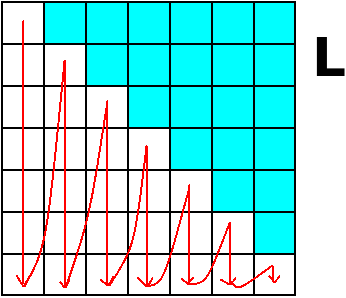
\includegraphics[scale=1]{cholesky.png}


Pero para que esto tenga sentido debemos tener $a_{kk} - \displaystyle \sum_{j=1}^{k-1} l_{kj}^2>0$ pues queremos que $l_{kk}$ sea real y distinto de cero así podemos dividir por él. \bigskip


Probemos que esto sucede, por inducción.

Sabemos que como $A$ es simétrica y definida postiiva todos los menores principales son positivos.\\

Si $k=1$ como $a_{11}>0$ ya está.\\

Supongamos que $l_{11},...,l_{k-1}{k-1}$ son todos distintos de cero.

%, pero que $a_{kk} - \displaystyle \sum_{j=1}^{k-1} l_{kj}^2>0 \leq 0$. Entonces $l_{kk}=0$ ó $l_{kk}$ es complejo no real.

Definamos $l_{kk}$ aunque sea $0$ o un número complejo.

Es fácil ver (con un dibujito) que si nos quedamos con los menores principales de $A$ y de $L$ entonces $A_k = L_k {L_k}^t$.


Tomando determinante obtenemos $0<det(A_k) = det(L_k)^2 = l_{11}^2...l_{k-1}{k-1}^2\ l_{kk}^2$. Como los primeros son todos positivos, $l_{kk}^2$ positivo. Luego $l_kk$ debe ser real distinto de cero.


%Hay que demostrar que $a_kk - sum_{j=1}^{k-1}l_{kj}^2$ es mayor o igual que cero. Esto se hace inductivamente, usando que se puede hacer la descomposicion para tamaños mas chicos y que los menores principales de la matriz son positivos.

\subsection{Métodos iterativos}


\begin{itemize}
    \item \textbf{Jacobi}
El método de Jacobi consiste en generar $x_{i}^{k+1}$ a partir de la ecuacion i-esima.


$x_i^{k+1} = \frac{b_i- \displaystyle \sum_{j=1}^{i-1}a_{ij}x_j^k - \displaystyle \sum_{j={i+1}}^{N}a_{ij}x_j^k }{a_ii}$

La escritura matricial es $x^{k+1}=-D^{-1}(L+U)x^k + D^{-1} b$ (y resulta facil de deducir de la definicion)

\item \textbf{Gauss Seidel} Este método resulta de cambiar los $x_j^k$ por $x_j^{k+1}$ para $j<i$:


$x_i^{k+1} = \frac{b_i- \displaystyle \sum_{j=1}^{i-1}a_{ij}x_j^{k+1} - \displaystyle \sum_{j={i+1}}^{N}a_{ij}x_j^{k} }{a_{ii}}$

Resulta conveniente utilizar las componentes anteriores para calcular $x^{k+1}$ solo se necesita tener un vector de memoria pues este comienza conteniendo a $x^{k}$ se va reescribiendo a medida que se calculan las componentes del vector $x^{k+1}$


La escritura matricial es $x^{k+1}=-(D+L)^{-1}Ux^k + (D+L)^{-1} b$.

Esto se deduce de la igualdad de arriba, pues tenemos 

$a_{ii} x_i^{k+1} = b_i- \displaystyle \sum_{j=1}^{i-1}a_{ij}x_j^k $

$\displaystyle \sum_{j=1}^{i-1}a_{ij}x_j^{k+1}
 + a_{ii} x_i^{k+1} = b_i- \displaystyle \sum_{j=i+1}^{N}a_{ij}x_j^k $
 
 $(L+D) x^{k+1} = b - U x_k$
 
 $x^{k+1} = (L+D)^{-1} b - (L+D)^{-1} U x_k$ 

\end{itemize}

Tambien se puede ver facilmente cual es la matriz de cada método que indica el error. Lo hago para Jacobi:

Se tiene $x=-D^{-1}(L+U)x + D^{-1} b$ luego $e^{k+1} :=x-x+1 = -D^{-1}(L+U) e^k = B_J e^k$ y tenemos $e^k = B_J^k e_0$.

Para que el método converja, entonces, queremos que $B^k$ tienda a cero. Una condicion suficiente aunque no necesaria es que exista alguna norma tal que $||B||<1$


\begin{observation}
    Si $B$ es simetrica el teorema que dice que basta analizar $\rho(A)$ resulta intuitivo, pues $\exists S$ tal que $B=SDS^{-1}$ y de esta igualdad se ve que $B^k$ tiende a cero si y solo si los autovalores de $A$ son todos menores que 1.    
\end{observation}




\begin{theorem}
    $\rho{A} = inf ||A||$
\end{theorem}

\begin{caution}
	$\rho$ es el supremo de los autovalores de la matriz, \textbf{incluyendo los complejos}.
\end{caution}

\begin{proof}
    Primero veamos que para toda norma, $\rho{A} \leq ||A||$. En efecto, esto se ve tomando un autovector $v$ de norma 1 de autovalor maximo $\lambda_{max}$. $|| A v || = |\lambda_{max}| ||v||$, pero $|| A v ||\leq ||A||$ asi que estamos.
    
    
    Sea $\varepsilon > 0$. Quiero construirme una norma $||.||$ tal que $||A|| \leq \rho(A) + \varepsilon$.
    
    Esto se logra mirando la forma de Jordan de $A$ y cambiando la base para que los bloques de Jordan tengan $\varepsilon$ en vez de 1, y tomando la norma infinito en esa base. El resultado se obtiene al observar que $||A||$ es el maximo de la suma de las componentes de una fila de $A$.
\end{proof}


\begin{corollary}
    $B^k \to 0 \Leftrightarrow \rho(B) < 1$
\end{corollary}

\begin{proof}
    La vuelta es facil ya que me construyo una norma.
    
    Veamos la idea, por contrarreciproco. Si $\rho(B) \geq 1$ entonces existe $z \in \mathbb{C}^n$ autovector de norma 1 de autovalor maximo. Luego $||B^k||\geq||B^k z|| = \rho(B)^k ||z||$. Tomando parte real e imaginaria se concluye lo deseado.
\end{proof}


Hay una demostracion alternativa, mas directa, de la vuela del corolario anterior. Consiste en pasar a $B$ a su forma de Jordan: $CBC^{-1} = J$. Ahora multiplicamos a izquierda por $D$ y a derecha por $D^{-1}$ siendo D la matriz diagonal que en el lugar $i,i$ tiene $\varepsilon^{-i}$.

\begin{caution} En este caso $D J D^{-1} \neq D D^{-1} J$. Es decir, \textbf{no} conmuta. En general el producto conmuta si una matriz es $\lambda Id$, que no es el caso.
\end{caution}

Queda una matriz como de Jordan pero con $\varepsilon$ en vez de unos. En realidad es la misma demostracion de arriba.

Ahora, sea $A = DCBC^{-1}D^{-1}$. Sea $S := DC$

$B^k = S^{-1}A^kS$ y entonces $||B^k||_\infty \leq Cond(S) ||A^k||_\infty \leq Cond(S) (\rho(B) + \varepsilon)^k \to 0$ si $\varepsilon$ cumple que $\rho(B)+\varepsilon <1$

\begin{observation}
	Conviene entender $||A B||_\infty \leq ||A|| ||B||_\infty$ olvidándose de qué norma es, solo usando que proviene de una norma de vectores.
	
	En efecto, si se la entiende como el supremo de $Av$ para $||v||_\infty = 1$ la desigualdad resulta más clara.
\end{observation}


\begin{theorem}
    $||B^k||^{1/k} \to \rho(B)$
\end{theorem}


\begin{proof}
    Basta hacerlo para la norma infinito porque todas las normas son equivalentes y elevar a $1/k$ mata a las constantes $c_1$ y $c_2$ de la equivalencia de normas.
    
    
    Tenemos $||B^k||_\infty \leq  Cond(S) (\rho(B) + \varepsilon)^k$. Hagamos aparecer $\rho(B)^k$ a la izquierda.
    
    $\rho(B)^k \leq \rho(B^k)$ (no vale la igualdad: pensar en una TL que en un subespacio sea una rotacion de grado $\pi/2$ y en el ortogonal sea diagonalizable con autovalores menores que 1. $B^4$ tiene a 1 como autovalor.
    
    Sigamos: $\rho(B)^k \leq \rho(B^k) \leq ||B^k||_\infty$ por magia lineal. Luego:
    
    $\rho(B)^k \leq  ||B^k||_\infty \leq  Cond(S) (\rho(B) + \varepsilon)^k$
    
    Entonces, elevando a $1/k$, tenemos: $\rho(B) \leq  ||B^k||_\infty^{1/k} \leq  Cond(S)^{1/k} (\rho(B) + \varepsilon) \to \rho(B) + \varepsilon$ porque como $S$ es inversible su condición es $\neq$ 0. Y medio que ya estamos, porque $\varepsilon$ era arbitrario.
\end{proof}

\begin{observation}
	Esto dice que $||B^k||$ se comporta igual que $\rho(B)^k$ para $k$ grande. Luego una forma de comparar métodos es comparar el radio espectral de las matrices de iteración.
\end{observation}

\begin{theorem}
	Si $A$ es simétrica y definida positiva entonces Gauss-Seidel converge 
\end{theorem}

\begin{proof}
	
\includegraphics[scale=0.5]{noproof.jpg}
	
	(no se vio en la teórica. Ojo que fue la cursada del 2do cuatri del 2017)
\end{proof}


\subsection*{Teorema de Gershgorin}

\begin{theorem}
%El \displaystyle es para que aparezca justo abajo
	Sean $A \in \C^{n\times n}$, $R_i = \displaystyle \sum_{j \neq i} |a_{ij}|$ la suma de los elementos de la columna $i$ que no son $a_{ii}$, y definamos el disco $D(a_{ii},R_i) = \{z \in  \C : |z- a_{ii}| \leq R_i\}$ . Si $\lambda$ es autovalor de $A$ entonces $\exists i$ tal que $\lambda \in D(a_{ii},R_i)$
\end{theorem}

Antes de la demo, un ejemplo:

\[
A=
  \begin{bmatrix}
    1 & 2 \\
    1 & -1
  \end{bmatrix}
\]

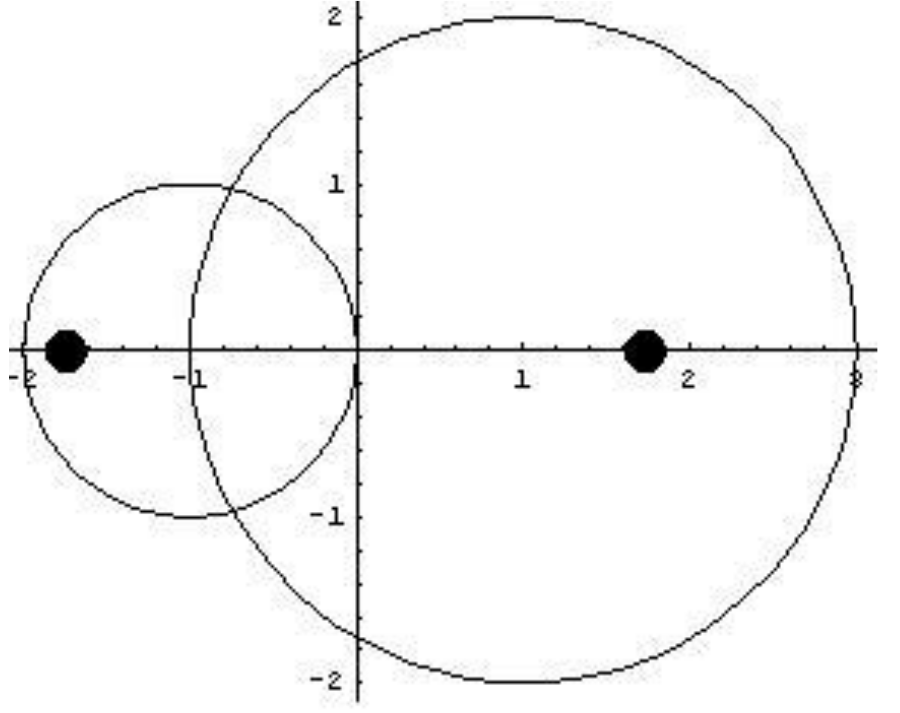
\includegraphics[scale=0.4]{gershgorin.png}
\captionof{figure}{Los nodos negros son los autovalores. Imagen obtenida de \href{https://goo.gl/qrSPf9}{Gershgorin’s Theorem for Estimating Eigenvalues}, de Sean Brakken-Thal}
\begin{proof}
	Sea $\lambda$ autovalor de $A$; tomo $v$ autovector de ese autovalor.
	Entonces tenemos $Av = \lambda v$, es decir:
	
% El align* le saca la enumeracion
\begin{align*}
\displaystyle \sum_{j=1}^n a_{1j} v_j = \lambda v_1\\
\displaystyle \sum_{j=1}^n a_{2j} v_j = \lambda v_2\\
\begin{gathered}
...
\end{gathered}\\
\displaystyle \sum_{j=1}^n a_{nj} v_j = \lambda v_n
\end{align*}

Queremos probar que $\exists i$ tal que $|\lambda - a_{ii}| \leq \displaystyle \sum_{j \neq i} |a_{ij}|$. ¿Cómo hacemos para deshacernos de $v$? Pidiendo que $||v||_\infty = 1$. Sea $i$ tal que $v_i = 1$, la coordenada que realiza la norma infinito. SPG supongamos $i=1$. Entonces tenemos $\displaystyle \sum_{j=1}^n a_{1j} = \lambda$. Pasando restando $a_{ii}$ obtenemos $\lambda - a_{ii} = \displaystyle \sum_{j \neq i} a_{ij}$. Enchufemos módulo: $|\lambda - a_{ii}| = |\displaystyle \sum_{j \neq i} a_{ij}| \leq \displaystyle \sum_{j \neq i} |a_{ij}|$, como queríamos ver.

\end{proof}

\begin{corollary}
	El teorema de Gershgorin nos permite probar el siguiente lema usado en la construcción de los splines cúbicos:
	
	Si $A$ es estrictamente diagonal dominante entonces es inversible.
\end{corollary}

\begin{proof}
	$\forall i, a_{ii} > \displaystyle \sum_{j \neq i} |a_{ij}| \Rightarrow |a_{ii} - \displaystyle \sum_{j \neq i} |a_{ij}| | > 0$. Luego $0 \not\in D(a_{ii},R_i) \Rightarrow 0$ (por la definición de los discos). Luego no puede ser autovalor.
	
	Notemos que hay una demostración alternativa, cuya idea pasa ligeramente por la demostración del teorema de Gershgorin. Consiste en suponer que $\exists v$ tal que $Av = 0$. Sea $i$ tal que $v_i$ es máximo.
	
	Tenemos que $ a_{ii} v_i = - \displaystyle \sum_{j \neq i} a_{ij} v_j \Rightarrow a_{ii} = - \displaystyle \sum_{j \neq i} a_{ij} \frac{v_j}{v_i}$
	
	Tomando módulo y acotando queda $|a_{ii}|  = | \displaystyle \sum_{j \neq i} a_{ij} \frac{v_j}{v_i} | \leq \displaystyle \sum_{j \neq i} |a_{ij}| |\frac{v_j}{v_i}| \leq \displaystyle \sum_{j \neq i} |a_{ij}| 1$, absurdo, pues $A$ era estrictamente diagonal dominante.
\end{proof}


\section{Normas y condicionamiento de matrices}
{
	Cuando queremos resolver $Ax=b$, para $b$ dato, como estamos en la vida real, puede pasar que al medir el dato haya un error. ¿Cómo afecta el error en el dato al error en la solución? Si reemplazamos $b$ por $b + \Delta b$ tendremos $A(x+\Delta x) = b + \Delta b$ para cierto $\Delta x$. Despejando, queda $A \Delta x = \Delta b$. \\
	
	Como los errores se suelen estudiar \textit{relativos}, porque no es lo mismo trabajar con $x ~ 10^4$ que $x~10^{-4}$, analizaremos $\frac{||\Delta x ||}{||x||}$. \\
	%TODO no se usar la ~
	%TODO rellenar!
	
	Definimos $Cond(A) = ||A|| ||A^{-1}||$. \\
	
	%TODO: usar theorem y esas cosas...
	Teorema: $\frac{||\Delta x|| }{||x||} \leq Cond(A) \frac{||\Delta b|| }{||b||}$\\
	
	O sea que cuanto más chico sea $Cond(A)$ mejor. Obs: $Cond(A) \geq 1$.
	
	Además vale la igualdad para algún $b$ y $\Delta b$ y además $\frac{1}{Cond(A)} \frac{||\Delta b ||}{||b||} \leq \frac{||\Delta x ||}{||x||}$
	
demostración	: es casi directa.

$\Delta x = A^{-1} \Delta b$ así que: \\

$\frac{||\Delta x||}{||x||} = \frac{||A^{-1} \Delta b||}{||x||} \leq \frac{||A^{-1}|| ||\Delta b||}{||x||}$. Ahora bien, queremos que aparezca $||b||$ así que lo hacemos aparecer multiplicando por $1$. Queda: \\

$\frac{||\Delta x||}{||x||} \leq \frac{||A^{-1}|| ||\Delta b||}{||x||} \frac{||b||}{||b||} = ||A^{-1}|| \frac{||\Delta b||}{||b||} \frac{||b||}{||x||}$, pero $b = Ax \Rightarrow$ puedo acotar $\frac{||b||}{||x||}$ por $||A||$, y obtenemos lo que queríamos. \\

Si tomamos $\Delta b$ que realice la norma de $A^{-1}$ y $b$ que realice la norma de $A$, las desigualdades se convierten en igualdades.


Para ver la otra afirmación, basta probar que $\frac{||\Delta b ||}{||b||} \leq Cond(A) \frac{||\Delta x ||}{||x||}$ (usando que $Cond(A)^{-1} = Cond(A)$ y aplicando el teorema a $A^{-1}$.

---------------------

La condición de una matriz también está involucrada con la propagación del error que se cometa en los coeficientes del sistema. \\


\begin{theorem}Si $A$ inversible, $E$ matriz, $Ax=b$ y $(A+E)(x+\Delta x) = b$ entonces llamando $\hat{x}=x+\Delta x$, tenemos:

$\frac{\Delta x}{\hat{x}}\leq Cond(A) \frac{||E||}{||A||}$,

Observemos que cambiamos $x$ por $\hat{x}$ y eso puede llegar a confundir a la hora de acordarse el teorema.

Además, si $Cond(A) \frac{||E||}{||A||}\leq \delta < 1$ entonces:

$\frac{\Delta x}{x}\leq \frac{1}{1-\delta}Cond(A) \frac{||E||}{||A||}$, es decir, recuperamos el $x$.
\end{theorem}


\begin{proof}
Observemos primero que $A \hat{x} = b - E \hat{x} \Rightarrow E \hat{x}= b - A \hat{x} = - A\Delta x$

Luego tenemos $||\Delta x|| = ||A^{-1} A \Delta x|| = ||A^{-1} E \hat{x}|| \leq ||A^{-1}|| ||E|| ||\hat{x}||$. Multiplicando y dividiendo por $||A||$ se obtiene lo deseado.



Ahora, si $Cond(A) \frac{||E||}{||A||}\leq \delta < 1$, hagamos lo siguiente:

$\frac{||\hat{x}||}{||x||} = 1 + \frac{||\Delta x||}{||x||}$, entonces:

$\frac{||\Delta x||}{||x||} \leq Cond(A) \frac{||E||}{||A||}(1 + \frac{||\Delta x||}{||x||})$ y listo.
\end{proof}

\begin{proposition}

$\displaystyle ||A||_1 = \underset{1\leq j \leq n}{max} \sum_{i=1}^n |a_{ij}|$

\end{proposition}

\begin{proof}
	Sea $||v||_1 = 1$. Luego $||Av||_1 \leq \displaystyle \sum_i \sum_j | a_{ij}| v_j$. Reordenando, obtengo $||Av||_1 \leq \displaystyle \sum_j |v_j| \displaystyle \sum_i |a_{ij}| \leq  \sum_j |v_j| \cdot \underset{1\leq j \leq n}{max} \sum_i |a_{ij}| = 1 \cdot \underset{1\leq j \leq n}{max} \sum_i |a_{ij}|$. Para ver que realiza la norma basta ver que si $j_0$ es la columna de suma de módulos máxima, $e_{j_0}$ cumple $||e_{j_0}||_1 = 1$ y $Ae_{j_0}$ realiza la norma.
\end{proof}

%TODO faltan ver algunos teoremas de normas de matrices.

%TODO tengo que hacer la norma 1

%TODO revisar teorema de rho < 1 entonces converge



\section{Métodos iterativos para resolver sistemas lineales}

Primero, una cuenta explicando cómo es Gauss-Seidel.

La idea de Jacobi era despejar la coordenada iésima del nuevo vector a partir de la iésima ecuación. La idea de Gauss Seidel es aprovechar los cálculos hechos hasta ahora.

Luego definimos $x_i^{k+1}=\frac{b_i - \displaystyle \sum_{j=1}^{i-1}a_{ij}x_j^{k+1}-\displaystyle \sum_{j=1}^{i-1}a_{ij}x_j^{k}}{a_{ii}}$\\

Si pasamos multiplicando $a_ii$ y sumando la primer sumatoria, obtenemos la siguiente igualdad:

$a_{ii} x_i^{k+1} + \displaystyle \sum_{j=1}^{i-1}a_{ij}x_j^{k+1} =  b_i - \displaystyle \sum_{j=1}^{i-1} a_{ij} x_j^{k}$\\

Juntando, obtenemos lo siguiente:

$\displaystyle \sum_{j=1}^{i}a_{ij}x_j^{k+1} =  b_i - \displaystyle \sum_{j=1}^{i-1} a_{ij} x_j^{k}$\\

Expresemos esto en forma matricial:

$(L+D) x^{k+1} = b - U x_k$. O sea:\\

$x^{k+1} = - (L+D)^{-1} U x_k + (L+D)^{-1} b$\\

Es decir, obtuvimos que $B_{GS} = - (L+D)^{-1} U$. Fantástico.

-----------------------------


\begin{definition}Una matriz A se dice estrictamente diagonal dominante si $|a_{ii}| > \displaystyle \sum_{j\neq i} |a_{ij}|$
\end{definition}

\begin{theorem}Si A es estrictamente diagonal dominante, ambos métodos convergentes
\end{theorem}

\begin{proof}
\textbf{Jacobi}: basta ver que $||B_J||_{\infty}<1$

Recordemos que $B_J = -D^{-1}(L+U)$, es decir,\\

$b_{ij}=-\frac{a{ij}}{a_{ii}}$ para $i\neq j$ y $b_{ii}=0$

Luego $||B_J||_{\infty} = \underset{i}{max} \frac{\displaystyle \sum_{j\neq i} |a_{ij}|}{|a_{ii}|}<1$ pues $A$ es diagonal dominante. \bigskip

\textbf{Gauss-Seidel} Este es un poquito más triqui, y vamos a necesitar probar que $\rho(B)<1$.

$B_{GS} = - (L+D)^{-1} U$

Sea $||x||_\infty=1$ autovector de autovalor $\lambda$. Luego $- (L+D)^{-1} Ux = \lambda x$. Como no sé manejar bien inversas, la paso para el otro lado, quedando:

$-Ux = \lambda (L+D) x$

Es decir, para cada $i$ tenemos $- \displaystyle \sum_{j=i+1}^N a_{ij} x_j = \lambda \displaystyle \sum_{j=1}^i a_{ij} x_j$

Ahora bien, yo quiero acotar $\lambda$ por 1 usando que la matriz es diagonal dominante. Necesito que aparezcan solas tanto $\lambda$ como $a_ii$.

La igualdad de arriba se puede expresar también como $- \displaystyle \sum_{j=i+1}^N a_{ij} x_j = \lambda \displaystyle \sum_{j=1}^{i-1} a_{ij} x_j + \lambda a_{ii} x_i$. Es decir:\\

$\lambda a_{ii} x_i = - \displaystyle \sum_{j=i+1}^N a_{ij} x_j -  \lambda \displaystyle \sum_{j=1}^{i-1} a_{ij} x_j$

Como quiero acotar $\lambda$, no paso sumando el último término sino que primero meto módulo. Como quiero deshacerme de $x_i$ pido $i$ tal que $x_i$ realice la norma infinito. (Por lo tanto $|x_j|\leq |x_i|$ y también puedo deshacerme de ellos). Queda:

$|\lambda| |a_{ii}| \leq \displaystyle \sum_{j=i+1}^N |a_{ij}| + \lambda \displaystyle \sum_{j=1}^{i-1} |a_{ij}|$. Ahora si paso restando para juntar los lambda:

$|\lambda| |a_{ii}| -  \lambda \displaystyle \sum_{j=1}^{i-1} |a_{ij}|\leq \displaystyle \sum_{j=i+1}^N |a_{ij}|$\\

$|\lambda| (|a_{ii}| - \displaystyle \sum_{j=1}^{i-1} |a_{ij}|)\leq \displaystyle \sum_{j=i+1}^N |a_{ij}|$\\

$|\lambda| \leq \frac{\displaystyle \sum_{j=i+1}^N |a_{ij}|}{(|a_{ii}| - \displaystyle \sum_{j=1}^{i-1} |a_{ij}|)}<1$ pues A es estrictamente diagonal dominante\\

\end{proof}
-------------------


\subsection{Método de House Holder}

Queremos escribir $A=QR$, porque si queremos resolver $Ax = b$ esto es lo mismo que $QRx = b$ y podemos multiplicar por $Q^t$ a ambos lados para obtener $Rx = Q^t b$

La idea es buscar una $Q$ ortonormal tal que $Qa_1 = (\pm ||x||,0,...,0)^t$, donde $a_1$ es la primer columna de $A$, y luego hacer inducción.

Vamos a reflejar contra el hiperplano adecuado.


Primero entendamos cómo reflejar vectores contra un hiperplano.

Antes de eso, entendamos cómo proyectar contra un hiperplano.

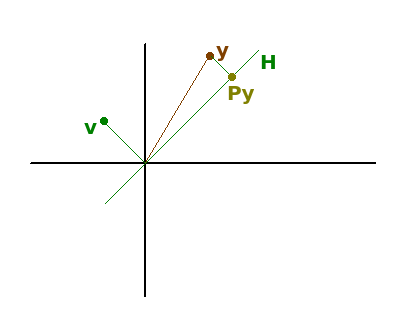
\includegraphics[scale=1]{householder1.png}
\caption{El esquema muestra la situación en $\R^2$}

Vale en general que $y=Py + <y,v> v$ donde $P$ es la proyección al hiperplano $H$. entonces, despejando, resulta $Py = y-v<v,y>$. Luego la proyección está dada por $P=Id-vv^t$.\\

Sea $||w||=1$. Entonces definimos $Q=Id-2ww^t$. El $2$ sale de que queremos reflejar. Es fácil chequear que $Q$ es ortogonal: $Q^t Q = (Id - 2 w w^t) (Id - 2 w w^t)$ pues $w w^t$ es simétrica.\\

Entonces $Q^t Q = Id - 4 w w^t + 4 w w^t w w^t$, pero $w^t w=||w||^2 = 1$ luego $Q^t Q = Id$, como queríamos ver. ¿Por qué queríamos ver esto? Porque queremos construirnos una $Q$ ortogonal tal que $Qa_1 = (\pm ||x||,0,...,0)^t$\\

Si en lugar de $w$ de norma 1 empezamos con un $v$ cualquiera, hay que arreglar las cosas. Primero observemos que la longitud del vector $v$ no influye en la reflexión, porque el hiperplano $H$ ortogonal a $v$ no cambia. Entonces, para reflejar contra $H$, podemos cambiar $v$ por $\frac{v}{||v||}$. Entonces podemos definir $Q$ de manera linda como $Q = Id - 2 \frac{v v^t}{v^t v}$ (ya que $v^t v = ||v||^2$).

Llamos $x=a_1$ para eliminar el subíndice.

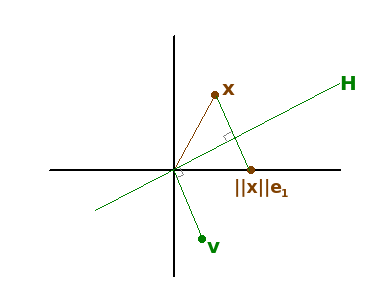
\includegraphics[scale=1]{householder3.png}

Observemos que $v$ debe ser paralelo a $x-||x||e_1$ si queremos que el resultado de reflejar a $x$ sea $||x||e_1$. Luego podemos tomar $v=x-||x||$, y $Q_1 = Id - 2 \frac{v_1 v_1^t}{v_1^t v_1}$\\

Una observación es que podríamos haber tomado $\hat{v} = - ||x||e_1 -x$ si queríamos reflejar a $x$ para que caiga en $-||x||e_1$ y también habría funcionado. En general, como no quiero restar cosas parecidas para que no haya cancelaciones catastróficas, voy a tomar $v= -sg(x_1)||x||e_1-x$, así $x_1$ y la primer coordenada de $-sg(x_1)||x||e_1$ tienen signos opuestos y por lo tanto están lejos.

\subsection*{Gram-Schmidt}

\begin{observation}
	Algo interesante es que también podemos obtener las matrices $Q$ y $R$ haciendo Gram-Schmidt. Si llamo $a_j$ a las columnas de $A$, la idea es que $Q$ sea los vectores obtenidos durante la ortonormalización de $A$.\\
	
	Definimos $R = Q^t A = (Q_i^t a_j)$. Observemos que si $i>j$ entonces $a_j$ es combinación lineal de $Q_1,...,Q_j$; por lo tanto $Q_i^t a_j = 0$. Luego $R$ es efectivamente triangular superior.\\
	
Ah, pero ¿quién dice que $QR = A$? ¡Esto hay que probarlo! $R = Q^t A \Rightarrow Q R = Q Q^t A = Id A = A$. Uff, qué susto.\\

Última observación: ¿Qué pasa si $A \in \mathbb{R}^{m\times n}$, con $m>n$? O sea, tiene más filas que columnas.\\

Gram-Schmidt puedo hacer alegremente, y también definir $R= Q^t A$.\\

Pero ojo, no es cierto que $QQ^t = Id$\\

Se puede ver ...

%TODO terminarlo

\end{observation}



%TODO escribirlo transpuesto

\begin{theorem}

 Si $A$ es simétrica y definida positiva entonces GS converge, pero Jacobi puede no converger (no fue demostrado)
\end{theorem}

\begin{proposition}Si $B=-M^{-1}N$ entonces $\lambda$ autovalor de $B$ si y solo si $det(\lambda M + N) = 0$
\end{proposition}

\begin{proof}

$det(\lambda Id - B) = 0 \Leftrightarrow det(\lambda Id + M^{-1}N ) = 0 \Leftrightarrow det(\lambda M + N) = 0$
\end{proof}

\begin{proposition}Si $A$ es tridiagonal entonces $\rho(B_{GS}) = \rho(B_J)^2$. En particular uno converge si y solo si el otro converge, aunque Gauss-Seidel resulta preferible. Otra observación es que en $\mathbb{R}^{2x2}$ toda matriz es tridiagonal.
\end{proposition}

\begin{proof}es cuestión de mirar los autovalores, sale solo.
\end{proof}


\begin{proposition}Si $B$ es diagonalizable con $\rho(B) \geq 1$ entonces $||e^k \to 0$ sii $e^0 \in gen\{\text{autovalores} < \text{1 en módulo} \}$
\end{proposition}
\begin{proof}

$\Leftarrow)$ fácil.

$\Rightarrow) e^k = \displaystyle \sum_{i=1}^n \alpha_i \lambda_i^k v_i$ con $v_i$ autovectores. El truco es considerar la norma 1 en la base de autovectores $||.||_*$ pues $||e^k||_* \to 0$ pero esto implica que $\alpha_i$ debe ser 0 para los $\lambda_i \geq 1$. (Se ve fácil que es una norma de vectores)

\end{proof}

\bigskip





\subsection{El método de gradiente}

La idea es que tenemos $f : \mathbb{R}^n \rightarrow \mathbb{R} C^1$ y queremos encontrar $x\in\mathbb{R}^n$ tal que $f(x)$ sea mínimo.

Sea $x^0$ inicial, busco $x^1 = x^0 + \alpha_0 d^0$ con $\alpha_0 \in\mathbb{R}, d^0 \in \mathbb{R}$. Es decir, me muevo en alguna dirección.

Por ejemplo, puedo elegir $d^0 = - \nabla f(x^0)$ para ir en la dirección en que $f$ más decrece.

En general, $x^{k+1} = x^k - \alpha_k \nabla(x^k)$.

Sea $A$ una matriz simétrica y definida positiva, busco una función $f$ tal que minimizar $f$ sea equivalente a solucionar $Ax=b$.

Una observación es que si me invento una $f$ cuadrática convexa, un mínimo local de $f$ va a ser un mínimo global de $f$, aunque todavía no sé por qué.\\

Sea $f(x) = \frac{1}{2} x^t A x - b^t x$\\

Si derivo y uso que $A$ es simétrica obtengo $\nabla f(x) = Ax -b$, como queríamos.\\

El método iterativo es de la forma $x^{k+1} = x^k - \alpha_k \nabla f(x_k) = x^k - \alpha_k(Ax^k-b)$. A la expresión $Ax^k-b$ se la llama residuo y se denota $r^k$, y $d^k = -r^k$. \\

Luego obtenemos $x^{k+1} = x^k + \alpha_k d^k$. Asumimos $d^k\neq0$\\

¿Cómo elegimos $\alpha_k$? Mirando $g(\alpha)=f(x^k + \alpha d^k$ y buscando un mínimo de g.

Derivando se obtiene $g'(\alpha_k) = 0 \Leftrightarrow \alpha_k = \frac{-r^k \cdot d^k}{d^k A d^k} = \frac{d^k \cdot d^k}{d^k A d^k}$

\textbf{Un caso más simple}: tomar $\alpha_k = \alpha$ constante.

Tenemos:\\

$x^{k+1}=x^k - \alpha(Ax^k-b)$\\
$x=x - \alpha(Ax-b)$\\

Restando se obtiene:\\

$e^{k+1} = x^{k+1} - x = x^k - x - \alpha A (x^k-x) = e^k - \alpha A e^k$ \\

Luego $e^k = (Id - \alpha A)^k e_0$, y pidiendo $\rho(Id-\alpha A)<1$ llego a que el método converge sii $\alpha < \frac{2}{\lambda_{max}}$


\textbf{Método del gradiente conjugado}

Quiero que las direcciones $d^k$ sean conjugadas, es decir, $d^i A d^j = 0\ \forall\ i\neq j$

Como antes, tomo $r^k = A x^k-b, \alpha_k = \frac{-r^k \cdot d^k}{d^k A d^k}$. Lo que va a cambair es la elección de $d^k$.

Tomo $d^{k+1} = - r^{k+1} + \beta_k d^k$ para que $d^{k+1}$ y $d^k$ sean conjugadas. (La cuenta sale fácil)

Queda que los residuos son todos ortogonales....pero esto no lo probaron.


\section{Interpolación}

Sea $P_n$ el conjunto de polinomios de grado menor o igual que $n$.

\subsection{Construcción}
\begin{theorem}Dados $n+1$ puntos existe un único polinomio $p\in P_n$ que los interpola a todos.
\end{theorem}

\begin{proof}

Unicidad: si $p$ y $q$ son dos polinomios que cumplen lo dicho anteriormente entonces $p-q$ tiene $n+1$ raíces y es de grado menor o igual que $n$ entonces es el polinomio 0.


Existencia: \\

Manera 1: con la base de Lagrange.

Manera 2: se pueden buscar coeficientes $(a_0,a_1,...,a_n)$ que sean solución de $V(x_0,...,x_n) a = y$.

Lo que debemos probar es que la matriz de Vandermonde es inversible. En efecto, veamos que su núcleo es trivial. Sea $(a_1,...,a_n) \in Nu V$ entonces las $n+1$ igualdades me dicen que el polinomio asociado tiene $n+1$ raíces distintas luego es el polinomio cero luego $a=0$ como vector. Es interesante notar que la unicidad y la existencia se prueban de igual manera si usamos coeficientes indeterminados.


\end{proof}

\subsection{Error de interpolación}

Llamamos $E_n(x) = f(x) - p_n(x)$

Definición: $W_{n+1}(x)=(x-x_0)...(x-x_n)$


\begin{theorem} En las condiciones de antes, para cada $x \in [a,b] \exists \xi=\xi(x)$ tal que $E_n(x) = \frac{f^{n+1}(\xi)}{(n+1)!} W_{n+1}(x)$

(Observemos el asunto molesto de que sea $E_n$ pero $W_{n+1}$)\\

\end{theorem}

\begin{proof}la idea es usar Rolle muchas veces en una función que tiene $f(x)-p_n(x)$ como constante.


Sea $F(t) = f(t) - p_n(t) - (f(x) - p_n(x))$

Esta no funciona...queremos que F se anule en $n+2$ puntos,y $F$ solo se anula en $x$. Los otros $n+1$ candidatos naturales son $x_0,...,x_n$, así que agregamos $W_{n+1}$ en la expresión:

$F(t) = f(t) - p_n(t) - (f(x) - p_n(x)) W_{n+1}(t)$

Pero esta tampoco funciona porque $F$ deja de anularse en $x$, así que hay que dividir por $W_{n+1}(x)$ al final, quedando:

$F(t) = f(t) - p_n(t) - \frac{f(x)-p_n(x)}{W_{n+1}(x)} W_{n+1}(t)$. Si llamamos $\alpha = \frac{f(x)-p_n(x)}{W_{n+1}(x)}$, queda $F(t) = f(t) - p_n(t) - \alpha W_{n+1}(t)$

Ahora sí, $F$ tiene n+2 raíces, entonces por Rolle $F'$ tiene n+1 raíces, y así siguiendo hasta que $F^{(n+1)}$ tiene una raíz. Llamémosla $\xi$.\\

¿Cómo es $F^{(n+1)}$? Es un poco molesto derivar $W_{n+1}(t)$, pero mirémoslo más cómodamente. Se trata de un polinomio mónico de grado $n+1$. Al derivarlo queda un polinomio de grado $n$ con coeficiente principal $n+1$. La derivada k-ésima nos devolverá un polinomio de grado $n+1-k$ cuyo coeficiente principal será $(n+1)n(n-1)...(n+1-k)$. Fijalmente, la derivada n+1-ésima será un polinomio constane cuyo coeficiente principal será $(n+1)!$ Esto nos dice que:

$F^{(n+1)}(t) = f^{(n+1)}(t)- \alpha (n+1)!$ y por lo tanto $F^{(n+1)}(\xi)= 0 = f^{(n+1)}(\xi) - \alpha (n+1)!$. Recordando quién era $\alpha$ nos daremos cuenta que ya terminamos la demostración.

\end{proof}

\subsection{Forma de Newton}

Observemos que la forma de Lagrange tiene la desventaja que si queremos agregar un nuevo nodo, hay que calcular todo el polinomio de nuevo.

Este problema lo soluciona la forma de Newton, que aparentemente se puede ver como una generalización del polinomio de Taylor asociado a una función, aunque más que generalización para más bien una analogía notacional.


\begin{definition}(diferencias divididas):

$f[x_0,x_1]=\frac{f(x_1)-f(x_0)}{x_1-x_0}$\\

$f[x_0,x_1,x_2]=\frac{f[x_1,x_2]-f[x_0,x_1]}{x_2-x_0}$\\
Para $k>1$: $f[x_0,...,x_{k}]=\frac{f[x_1,..,x_{k}]-f[x_0,...,x_k]}{x_{k}-x_0}$
\end{definition}

Idea: construir $p_{k+1}(x) = p_k(x) + a_{k+1}(x-x_0)...(x-x_k)$ eligiendo $a_k$ acordemente.

Haciendo este procedimiento se obtiene la forma de Newton:

$p_n(x) = a_0 + a_1 (x-x_0) + a_2 (x-x_0)(x-x_1) + ... + a_n(x-x_0)...(x-x_n)$ \\

Lo interesante es que los $a_k$ son las diferencias divididas. Esto se puede ver por inducción. El caso n=1 es fácil.

$n\Rightarrow n+1: $ Sabemos que $p_n(x) = a_0 + a_1 (x-x_0) + a_2 (x-x_0)(x-x_1) + ... + a_n(x-x_0)...(x-x_n) $ interpola a $x_0,...,x_n$ y que 
$q_n(x) = b_0 + b_1 (x-x_1) + b_2 (x-x_1)(x-x_2) + ... + b_n(x-x_1)...(x-x_{n+1}) $ interpola a $x_1,...x_{n+1}$. Luego puedo definir:\\

$r(x) = \frac{(x-x_0) q_n(x) - (x-x_{n+1}) p_n(x)}{x_{n+1} - x_0}$, donde divido por esa diferencia para que $r(x)$ interpole a los $n+1$ puntos. Este polinomio tiene grado menor o igual  que $n+1$ (algún coeficiente podría ser 0). Pero entonces es el interpolador.

Si $r(x) = a_0 + a_1 (x-x_0) + a_2 (x-x_0)(x-x_1) + ... + a_{n+1}(x-x_0)...(x-x_{n+1})$ por HI ya sabemos que los $a_i$ con $i < n+1$ son lo que deben ser, es decir, las diferencias divididas, ya que como el nuevo término se anula al evaluarlo en los primeros $n$ puntos, si miro lso primeros $n$ términos de la expresión obtengo el interpolador en $x_0,...x_n$.

Entonces mirando $a_{n+1}$ se obtiene $a_{n+1}= f[x_0,...x_{n+1}]$, que era lo que queríamos.

Queda $p_n(x) = f(x_0) + f[x_0,x_1] (x-x_0) + ... + f[x_0,...,x_n] (x-x_0)...(x-x_n)$
----------------------

Volvamos a expresar el eerror de interpolación con esta nueva expresión.

\begin{theorem}si $p_n \in P_n$ interpola a $f$ en $x_0,...,x_n$ entonces se tiene $E_n(x) = f(x) - p_n(x) = f[x_0,...,x_n,x] W_{n+1}(x)$
\end{theorem}

\begin{proof} Para $x \neq x_i$ (sino trivial) consideramos $x_{n+1}:=x$ y consideramos el polinomio interpolador $p_{n+1}$ que interpola a la función en esos $n+2$ puntos.

Tenemos $f(x) = p_{n+1}(x) = p_n(x) + f[x_0,...,x_{n+1}]W_{n+1}(x_{n+1})$

Restando $p_n(x)$ obtenemos $E_n(x) = f[x_0,...,x_{n+1}]W_{n+1}(x_{n+1})$, como queríamos. ¡Aleluya!

\end{proof}

\subsection{Polinomios de Tchebychev - Minimización del Error}

Los polinomios de Tcheychev se definen como $T_k(x) = cos(k\ cos^{-1}x)$, para $x\in[-1,1]$. Una regla mnemotécnica podría ser que el $cos^{-1}$ se lo tenés que enchufar a alguien y el candidato natural es $x$ por vivir en $[-1,1]$ y que además tienen que aparecer un $k$ y un coseno.

Ahora bien, ¿cómo probamos que son polinomios? Por inducción + identidades trigonométricas.

Casos $k=1$,$k=2$ (Importante: ¡hay que hacerlos para poder hacer inducción bien!)

La única regla trigonométrica que me creo capaz de deducir es $cos(\alpha + \beta) = cos(\alpha) cos(\beta) - sen(\alpha) sen(\beta)$, porque me acuerdo la forma y voy probando en distintos valores.

Quiero aplicársela a $T_{k+1}$. Si llamo $\theta = cos^{-1}x$ tenemos $T_{k+1}(x) = cos((k+1)\theta) = cos((k+1)\theta + \theta)$

Si uso la regla trigonométrica me van a aparecer senos y no quiero eso en este contexto, pero $cos(\alpha - \beta) = cos(\alpha) cos(\beta) + sen(\alpha) sen(\beta)$ entonces $cos(\alpha + \beta) + cos(\alpha - \beta) = 2 cos(\alpha) cos(\beta)$ y eso es bueno porque entonces:\\

$T_{k+1}(x) = 2 cos((k \theta) cos(\theta) - cos(k \theta - \theta) $, pero $k \theta - \theta= (k-1) \theta$ con lo cuál $T_{k+1}(x) = 2x T_k(x) - T_{k-1}(x)$ y por HI concluimos que $T_{k+1}$ es un polinomio.


\begin{proposition}Sea $T_k$ el polinomio de Tchebyshev de grado k. Entonces:

(1) El coeficiente principal de $T_k$ es $2^{k-1} \forall k \in \mathbb{N}$

(2) Las raíces del polinomio $T_k$ se encuentran en el intervalo $[-1,1]$ (i.e. no son complejas) y son de la forma $x_i= cos(\frac{(2i+1)\pi}{2k})$ para $i=0,1,...,k-1$. En particular son todas distintas.

(3) $||T_k||_\infty = 1$. Además, $T_k$ alcanza los valores $1$ y $-1$ en $k+1$ puntos. (Y por lo tanto realiza su norma).

\end{proposition}

\begin{proof}

(1) Sale de la expresión $T_{k+1}(x) = 2x T_k(x) - T_{k-1}(x)$ a la que llegamos antes + inducción.

(2)  Sale de la expresión $T_k(x) = cos(k\ cos^{-1}x)$

(3) $|T_k(x)|\leq 1$ por ser imagen de la función coseno y además en $y_i = cos(\frac{i\pi}{k})$ alcanza los valores que queríamos, y de manera alternada. No lo hace en ningún otro punto.
\end{proof}

-----------------


Ahora sí, el teorema: \\

\begin{theorem}Entre todos los polinomios mónicos de grado $n+1, W_{n+1}(x) = \frac{1}{2^n} T_{n+1}(x)$ es el polinomio mónico que minimiza $||.||_\infty$ en $[-1,1]$
\end{theorem}

\begin{proof}

Supongamos que existe $P\in P_{n+1}$ mónico tal que $||P|| < ||W_{n+1}||$. Si restringimos $W_{n+1}$ a $[y_i,y_{i+1}]$, $W_{n+1}$ alcanza la norma infinito en cada subintervalo. Luego debemos tener $||P|| < \frac{1}{2^n} = ||W_{n+1}||$ en cada subintervalo. $W_{n+1}(y_i)$ se va alternando. Supongamos $W_{n+1}(y_i) = \frac{1}{2^n} > 0$ y $W_{n+1}(y_{i+1}) = \frac{-1}{2^n} < 0$ entonces necesariamente $P(y_i) < \frac{1}{2^n}$ y $P(y_{i+1}) < \frac{-1}{2^n}$

Luego $Q(x)= P(x) - W_{n+1}(x)$ tiene al menos un cero en $[y_i,y_{i+1}]$. Esto pasa en cada subintervalo; si $W_{n+1}(y_i)<0$ y $W_{n+1}(y_{i+1})>0$ es análogo.

Luego tenemos que $Q(x)$ tiene al menos $n+1$ raíces distintas. Pero es una resta de polinomios mónicos de grado menor o igual a $n+1$ así que tiene grado menor o igual a $n$. Absurdo! Luego tal polinomio no puede existir.\\

\end{proof}

Observación: puede demostrarse que si $P \neq W_{n+1}$ entonces la desigualdad de las normas es estricta (nosotros probamos por el absurdo que es un menor o igual).\\


Corolario: Si interpolamos a $f$ en las raíces de Chebychev podemos agregar un $2^n$ dividiendo.


Observación: una traslación nos permite dar los polinomios de Tchebyshev en $[a,b]$. Nosotros queremos $t(x)$ tal que $t(a) = -1$ y $t(b) =1$. Usando por ejemplo la forma de Lagrange llegamos a que $t = \frac{2(x-a)}{b-a} - 1$ y se llega a algo parecido a lo de antes con estos nuevos polinomios, usando que $\hat{T_k}(x)= T_k(t) = T_k(\frac{2(x-a)}{b-a} - 1)$

---------------

\begin{theorem} (Faber) Dados puntos\\

$\\
x_0^0\\
x_0^1 x_1^1\\
x_0^2 x_1^2 x_2^2\\
...\\
$\\
arbitrarios en $[a,b]$, existe una función $f$ continua tal que $||f-p_n|| \not\to 0$
\end{theorem}

\subsection{Hermite}

Observación: no se pueden saltear derivadas.

Supongamos que queremos

%TODO escribirlo mejor

$p(x_0)=f(x_0), p'(x_0) = f'(x_0), p(x_1) = f(x_1), p'(x_1) = f'(x_1)$

podemos escribir $p_3(x)= a_0 + a_1 (x-x_0) + a_2 (x-x_0)^2 + a_3 (x-x_0)^2 (x-x_1)$ aprovechando que $\{1,x-x_0,(x-x_0)^2, (x-x_0)^ (x-x_1)\}$ es base por ser todos de distinto grado.

Al buscar los coeficientes y definir $f[x_0,x_0] :=f'(x_0)$ obtengo que $p_3(x)= f[x_0] + f[x_0,x_0] (x-x_0) + f[x_0,x_0,x_1] (x-x_0)^2 + f[x_0,x_0,x_1,x_1] (x-x_0)^2 (x-x_1)$, lo cual generaliza la forma de Newton permitiendo nodos repetidos.


\begin{observation}
	El polinomio de Taylor es un caso particular de interpolación de Hermite donde se interpola a $f,f',...,f^{(n)}$ en $x_0$. El error del polinomio de Taylor coincide con el error de Hermite.
\end{observation}

\subsection{Interpolación por polinomios a trozos, Splines cúbicos}

\begin{lemma}: si $A$ es estrictamente diagonal dominante entonces es inversible.
\end{lemma}
\begin{proof}
	Es un corolario del teorema de Gershgorin, demostrada después.
\end{proof}
%TODO hacer

\begin{theorem} Dada $f \in C[a,b]$ y $a = x_0 < x_1 < x_2 ... < x_n = b$ existe una única $S \in C^2[a,b]$ tal que $S(x_j)=f(x_j \forall 0\leq j \leq n$, S es cúbica en cada intervalo, y $S''(a) = S''(b)=0$.
\end{theorem}

Las últimas dos condiciones se piden porque sobran. Fijémonos que si hay $n+1$ puntos el spline está compuesto por $n$ cúbicas $S_j$, con $0\leq j < n$.

Queremos lo siguiente:

\begin{itemize}
	\item $S_j(x_j)\ \forall\ 0 \leq j < n$
	\item $S(x_{j+1}) = f(x_{j+1})$
	\item $S_j(x_{j+1}) = S_{j+1}(x_{j+1})\ \forall\ 0 \leq j < n$ así el spline queda continuo
	\item $S_j'(x_{j+1}) = S_{j+1}'(x_{j+1})\ \forall\ 0 \leq j < n$ así es $C^1$
	\item $S_j'(x_{j+1}) = S_{j+1}'(x_{j+1})\ \forall\ 0 \leq j < n$ así es $C^2$
\end{itemize}

Es medio engorroso escribirlo de esta manera, porque la segunda condición queda colgada. Pero observemos que esto queda equivalente a:


\begin{itemize}
	\item $S_j(x_j)\ \forall\ 0 \leq j < n$
	%TODO escribir en negrita el cambio f(x_{j+1})
	\item $S_j(x_{j+1}) = f(x_{j+1})\ \forall\ 0 \leq j < n$ así el spline queda continuo y además $S_{n-1}$ interpola a $f$ en $x_{j+1}$
	\item $S_j'(x_{j+1}) = S_{j+1}'(x_{j+1})\ \forall\ 0 \leq j < n-1$ así es $C^1$
	\item $S_j'(x_{j+1}) = S_{j+1}'(x_{j+1})\ \forall\ 0 \leq j < n-1$ así es $C^2$
\end{itemize}

Luego efectivamente hay $n+n+(n-1) + (n-1) = 4n-2$ condiciones para $n$ polinomios de grado 3, que tienen $4$ coeficientes cada uno. Luego tengo $4n$ coeficientes a determinar y $4n-2$ condiciones, así que puedo agregar 2 condiciones arbitrarias, como esas $2$ del teorema. 

Notemos $S_j$ a $S$ restringida al subintervalo correspondiente y $h_j = x_{j+1} - x_j$

$S''$ debe ser una poligonal. Se tiene:\\

$S''_j(x) = y_j \frac{x_{j+1}-x}{h_j}+ y_{j+1} \frac{x-x_j}{h_j}$\\

Integrando dos veces aparecen constantes de integración $c_j$ y $d_j$ que usamos para que se verifiquen las otras condiciones. A las $y_j$ las elegimos para que $S'$ resulte continua.\\

Queda un sistema lineal tridiagonal estrictamente dominante que por lo tanto es inversible. (Ver apunte de la materia)\\

Notemos que en esta demostración se necesita una buena notación porque sino queda un enchastre.

\section{Aproximación por cuadrados mínimos}

\begin{theorem} (Desigualdad de Schwarz): Sea $V$ un espacio vectorial sobre $\mathbb{R}$ con producto interno. Entonces $\forall x,y \in V |<x,y>| \leq ||x|| ||y||$\\
\end{theorem}


%TODO HACER HOUSEHOLDER
\begin{proof}$\forall t\in\mathbb{R}$ sabemos que $<x+ty,x+ty> \geq 0$\\

Esto es equivalente a que $||x||^2 + 2t<x,y> + t^2 ||y||^2 \geq 0$. Si fijamos $x,y$ obtenemos una cuadrática en $t$ que es $\geq 0$ siempre luego su discriminante es $\leq 0$, es decir, $4<x,y>^2 - 4 ||y||^2 ||x||^2 \leq 0$ entonces $|<x,y>| \leq ||x|| ||y||$. Muy lindo.\\
\end{proof}
-------------------------

\begin{theorem} Sea V un e.v.p.i. y $S \subset V$ subespacio. Dado $x\in V$, $y\in S$, son equivalentes:
\\
1. $||x-y|| \leq ||x-s||\ \forall s\in S$\\
2. $<x-y,s> = 0\ \forall s\in S$\\

Además, $y$ es único.
\end{theorem}

\begin{proof}$1 \Rightarrow 2)$: planteando $g(t)=||x-(y+ts)||^2$. Sabemos que debe ser $g'(0)=0$. Derivando y evaluando en $0$ obtenemos 2.\\

Otra manera: Como $y-s \in S$, tenemos que $||x-y||^2 \leq ||x-(y+s)||^2 = ||(x-y) - s||^2 = ||x-y||^2 -2<x-y,s> + ||s||^2$. Tachango queda $2<x-y,s> \leq ||s||^2$. Cambiando $s$ por $t\ s$, donde $t\in\R$, obtenemos $2t<x-y,s> \leq t^2 ||s||^2$. Haciendo el límite cuando $t \to 0$ por izquierda y por derecha obtenemos lo deseado.

$2 \Rightarrow 1)$: Sale acotando para abajo, mirá qué bien: $||x-s||^2 = ||x-y+y-s||^2 = ||(x-y)+(y-s)||^2 = ||x-y||^2 + ||y-s||^2 \geq ||x-y||^2$\\

Unicidad: supongamos $y,\hat{y}$ cumplen lo pedido entonces $<\hat{y}-y,s>=0 \forall s\in S$ pero tomando $s = \hat{y}-y$ estamos.
\end{proof}

Para la existencia nos conseguimos una base ortonormal, hacemos la proyección y vemos que se cumple (2).


-------------------------

En el caso básico de polinomios y puntos en el espacio, el problema se puede llevar a minimizar $||Ax-b||$.\\

\begin{theorem}: Son equivalentes:
\\
(1) $x_0 \in \mathbb{R}^n minimiza ||Ax-b||$\\
(2) $x_0$ es solución del sistema $A^tA x = A^t b$
\end{theorem}


\begin{proof}
¿Qué queremos minimizar? Queremos $x_0$ tal que $||A x_0 - b || \leq ||A x - b|| \forall x \in \mathbb{R}^n$

Esto sucede si y solo si $<b - A x_0, A x > = 0 \forall x \in \mathbb{R}^n$. Paso $A$ para el otro lado y esta condición queda equivalente a

$<A^tb - A^t A x_0, x> = 0 \forall x \in \mathbb{R}^n \Leftrightarrow A^tb - A^t A x_0 = 0$

Una condición suficiente para que haya solución (aunque realmente no sé si es necesaria) es que las columnas de $A$ sean L.I pues en ese caso tendría núcleo trivial y por lo tanto afirmo que $A^t A$ sería inversible, pues si $A^tAx=0$ entonces $<A^tAx,x> = 0$ y entonces $<Ax,Ax>=0$ entonces $x=0$. (Y por lo tanto habría solución del problema)

\end{proof}


\begin{theorem}Si la norma es integrar con pesos, entonces $||f-p_n^*|| \to 0$
\end{theorem}

\begin{proof}
Sea $\varepsilon > 0$ entonces $\exists p \in P_n$ tal que $||f-p||_\infty < \varepsilon$

Luego $||f-p_n^*||^2 \leq ||f-p||^2 \leq \varepsilon^2 \int_a^b w(x) dx$ \bigskip
\end{proof}

\begin{corollary}(Igualdad de Parseval): para un producto interno como el del teorema anterior se tiene $||f||^2 = \displaystyle \sum_{j=0}^\infty <f,p_j>^2$
\end{corollary}

\begin{proof}

$||p_n^*||^2 = \displaystyle \sum_{j=0}^n <f,p_j>^2$

Luego $||f||^2 = ||f-p_n^*||^2 + ||p_n^*||^2$. Tendiendo $n$ a infinito se obtiene lo deseado.
\end{proof}
--------------------------------

El siguiente teorema intenta dar una forma más eficiente de encontrar los polinomios ortogonales asociados a un producto interno.

\begin{theorem}

 si vale $<xf,g> = <f,xg>$ entonces los polinomios ortogonales mónicos satisfacen la siguiente relación de recurrencia:\\

$q_n(x) = (x-a_n) q_{n-1} - b_n q_{n-2}(x) \forall n \geq 2$ 
\\
donde $a_n=$ "algo" y $b_n=$ "otra cosa"\\
\end{theorem}

\begin{proof}

Sea $n\geq 2$. Como 0 es raíz del polinomio $q_n(x) - q_n(0)$, podemos factorizar y escribir: $q_n(x) - q_n(0) = x r_{n-1}$\\

Podemos escribir $q_n(x) = x r_{n-1} + q_n(0)$. Intercalemos $x q_{n-1}$. Queda:
$q_n(x) = x q_{n-1} + x (r_{n-1}(x) - q_{n-1}(x)) + q_n(0)$\\

Un par de observaciones: $r_{n-1}$ tiene grado menor o igual que $n-1$ y es mónico. En realidad me parece claro que tiene grado exactamente $n-1$, pero nunca lo uso.\\

Además $x (r_{n-1}(x) - q_{n-1}(x)) \in P_{n-1}$ ya que los polinomios que estoy restando son mónicos y con la resta el grado baja.\\

Luego $\exists n\ \beta_j$ tal que $x (r_{n-1}(x) - q_{n-1}(x)) = \displaystyle \sum_{j=0}^{n-1} \beta_j q_j(x)$\\

Tenemos entonces que $q_n(x) = x q_{n-1}(x) + \displaystyle \sum_{j=0}^{n-1} \beta_j q_j(x)$\\

Si les hacemos producto interno contra $q_i$ con $i<n-2$ obtenemos:\\

$<q_n,q_i> = 0 = <x q_{n-1}, q_i> + \displaystyle \sum_{j=0}^{n-1} \beta_j <q_j,q_i>$. Pero por hipótesis $<x q_{n-1}, q_i> = <q_{n-1},x q_i>=0$ así que queda $0 = \beta_i \forall i<n-2$\\

Luego $q_n(x) = x q_{n-1}(x) + \beta_{n-1}\ q_{n-1}(x) + \beta_{n-2}\ q_{n-2}(x)$ 

¿Qué son esos $\beta$ que quedaron colgando?
Si haecmos $0=<q_n,q_{n-1}> = <x q_{n-1}, q_{n-1}> + \beta_{n-1} <q_{n-1},q_{n-1}>$ (recordemos que no son ortonormales) obtenemos cómo es $\beta_n$. Análogamente, obtenemos una expresión para $\beta_{n-2}$ si consideramos $0=<q_n,q_{n-1}>$

Se obtiene $-\beta_{n-2} = \frac{<x q_{n-1}, q_{n-2}>}{<q_{n-2},q_{n-2}}$. Ahora bien, esta expresión se puede mejorar (?), eliminando la $x$ del numerador.

$<x q_{n-1}, q_{n-2}> = <q_{n-1},x q_{n-2}>$

Ahora bien, $<q_{n-1},x\ q_{n-2}> - <q_{n-1},x\ q_{n-1}> = <q_{n-1},(x\ q_{n-2}- q_{n-1})>=0$ pues el polinomio del lado derecho tiene grado menor o igual a $n-2$ por ser una resta de mónicos de grado $n-1$ (¡el grado podría ser menor!).
\end{proof}


\section{Reglas de cuadratura}

\begin{proposition}
A partir de una regla de cuadratura $Q_0(f) = \displaystyle \sum_{j=1}^n A_j f(x_j)$ que aproxima $\int_{-1}^1$ se puede extraer una regla de cuadratura en $[a,b]$, que además resulta ser del mismo grado.

\end{proposition}

\begin{proof}
	Hay que hacer cambio de variables.
	
	Buscamos $[-1,1] \overset{\gamma(t)}{\rightarrow} [a,b]$ y hacemos $\underset{[a,b]}{\int} f(x) dx = \underset{\gamma^{-1}[a,b]}{\int} f\circ \gamma(t) \gamma'(t) dt$ y queda. Observar que como $\gamma$ es lineal el grado de exactitud no cambia.
\end{proof}

\begin{theorem}
	 Dada una regla de cuadratura $Q(f)$ que cumpla las siguientes condiciones razonables:
	 i) Es lineal\\
	 ii) Tiene grado de exactitud $k$\\
	 iii) $|Q(f)| \leq M (b-a) ||f||_\infty$ para alguna constante $M$,\\
	 
	 entonces si $f\in C^{k+1}[a,b]$, se tiene:\\
	 $|R(f)|=|I(f)-Q(f)| \leq \frac{(1+M) (b-a)^{k+2}}{(k+1)!} ||f^{k+1}||_\infty$
\end{theorem}

\begin{proof}
	La idea es hacer Taylor, sorprendentemente. Agarrando $p_k$ el polinomio de Taylor de grado $k$, obtenemos $||f-p_k||_\infty \leq \frac{(b-a)^{k+1}}{(k+1)!} ||f^{k+1}||_\infty$
	
	Ahora intercalemos $p_k$. Tenemos $I(f)-Q(f) = I(f) - I(p_k) + Q(p_k) - Q(f) = I(f-p_k) + Q(p_k - f)$.\\
	
	Pero entonces $|I(f)-Q(f)|\leq \frac{(b-a)^{k+2}}{(k+1)!} ||f^{k+1}||_\infty + M(b-a) ||f-p_k||_\infty \leq \frac{(b-a)^{k+2}}{(k+1)!} ||f^{k+1}||_\infty + M(b-a)  \frac{(b-a)^{k+1}}{(k+1)!} ||f^{k+1}||_\infty = (M+1) \frac{(b-a)^{k+2}}{(k+1)!} ||f^{k+1}||_\infty$
\end{proof}

\begin{theorem}
	Teorema del valor medio generalizado:
	
	Si tengo $\int_a^b h\circ\xi(x) g(x) dx$ con $h$ continua y $g$ no cambia de signo, entonces $\exists \eta \in [a,b]$ tal que 
	$h(\eta)=\int_a^b h\circ\xi(x) g(x) dx$
\end{theorem}

\begin{proof}
	Asumo $g\geq 0$, el otro caso es análogo.
	$h$ es continua entonces $\exists\ m,M$ tal que $m\leq h(y)\leq M$ Entonces $m\leq h\circ \xi(x) \leq M$ y por lo tanto, como $g$ no cambia de signo, $m g(x)\leq h\circ \xi(x) g(x)\leq M g(x)$\\
	
	Integrando, queda $m \int_a^b g(x) dx \leq \int_a^b h\circ \xi(x) dx \leq M \int_a^b g(x) dx$. Si $g$ es idénticamente cero el teorema es trivial, así que asumamos que no. Entonces puedo dividir por $\int_a^b g(x) dx$ y queda:
	
	$m \leq \frac{\int_a^b h\circ \xi(x) dx}{\int_a^b g(x) dx} \leq M$
	
	Como $h$ es continua, por el increíble teorema de Bolzano podemos concluir que existe $\eta$ tal que $h(\eta)=\frac{\int_a^b h\circ \xi(x) dx}{\int_a^b g(x) dx}$. Amazing.
\end{proof}

\begin{observation}
Esto nos permite hallar el error para la regla de trapecios cerrada, usando la fórmula del error del polinomio interpolador.

En efecto, queda $R(f) = \int_a^b \frac{f''(\xi)}{2} W_2(x) dx$ pero recordando que en este caso $W_2(x)=(x-a)(x-b)$, vemos que $W_2$ juega el rol de $g$ y no cambia de signo, luego $\exists \eta$ tal que $R(f) = \frac{f''(\eta)}{2} \int_a^b (x-a)(x-b) dx = - \frac{f''(\eta)}{12} (b-a)^3$


El caso del error de la regla de Simpson cerrada (integrar una cuadrática) es bastante más horrible.

Analicemos la regla de cuadratura en un intervalo $[-h,h]$ primero. En este caso $Q(f)=h\frac{1}{3}f(-h) + \frac{1}{3}f(0) + \frac{4}{3}f(h)$.

Definamos $F(x) = \int_0^x f(x) dx$ y $e(t) = F(t) - F(-t) - t[\frac{1}{3}f(-t) + \frac{1}{3} f(0) + \frac{4}{3} f(t)]$. La definimos así para que $R(f)=e(h)$

Encontremos una expresión para $e(h)$.

Derivando dos veces, obtenemos $e^{(3)}(t) = \frac{t}{3}[f^{(3)}(-t)-f^{(3)}(t)]$.\\

Entonces, por el teorema de valor medio, $\exists \xi_1 = \xi_1(t)$ tal que $e^{(3)}(t) = \frac{2t^2}{3} f^{(4)}(\xi_1)$.

Integremos:\\

$e^{(3)}(t) = \int_0^t \frac{2u^2}{3} f^{(4)}(\xi_1) du$

Ahora, aplicando TVM generalizado con $g=\frac{2t^2}{3}$ y observando que $e^{(3)}(0)=0$ obtenemos:

$e^{(2)}(t) = -\frac{2}{9} f^{(4)}(\xi_2)t^3$.

Iterando un par de veces el proceso llegamos a $e(h) = -\frac{5}{90}f^{(4)}(\eta)$.

Te creíste que habíamos terminado, pero todavía tenemos que dar una fórmula del error en $[a,b]$.

Pero observemos que podemos usar el cambio de variables para decir que $\int_a^b f(x) dx = \int_{-1}^1 \alpha f(\alpha t + \beta)$, con $\alpha = \frac{b-a}{2}$.

Luego el error de cuadratura de $f$ al integrar en $[a,b]$ es el error de $g(t)=\alpha f(\alpha t + \beta)$ en el $[0,1]$.

Derivando $g$ 4 veces y tomando $h=1$ queda $e(h) = \frac{-1}{90} (\frac{b-a}{2})^5$

\begin{caution}
	Podríamos acotar esos $f^(4)(\xi_i)$ por la norma infinito de $f^(4)$ pero entonces tendríamos un menor o igual, y está bueno tener una expresión para el error que sea una igualdad.
\end{caution}

\end{observation}


\subsection{Cuadratura Gaussiana}

\begin{theorem}
Consideremos el producto interno $<f,g>:= \int_a^b f(x) g(x) \omega(x) dx$. Si al hacer GS obtenemos ${p_j}$ los polinomios ortonormales, tenemos que las raíces de $p_n$ son todas distintas entre sí y pertenecen a $(a,b)$.
\end{theorem}

\begin{proof}
	Sea $n\geq 1$ fijo.
	
	(1) $p_n$ tiene al menos una raíz real. En efecto, si no fuera así, SPG podemos suponer $p_n >0$ en $(a,b)$. Pero $0=<1,p_n> = \int_a^b p_n(x) \omega(x) dx > 0$ Absurdo! Luego $p_n$ tiene al menos una raíz real.\\
	
	(2) $p_n$ no tiene raíces dobles. En efecto, supongamos que tiene un cero múltiple. Entonces $q(x) = \frac{p_n(x)}{(x-x_0)^2}$ es un polinomio de grado $n-2$ y por lo tanto ortogonal a $p_n$.
	
	Luego $0=<q,p_n> = \int_a^b (\frac{p_n}{(x-x_0)})^2 dx > 0$ absurdo nuevamente.
	
	(3) Si $x_0,...,x_k$ son las raíces de $p_n$ en $(a,b)$ entonces $k=n-1$. Supongamos que no, entonces $s(x) = (x-x_0)...(x-x_k)$ tiene grado menor que $n$ y por lo tanto $0=<s,p_n> = \int_a^b r(x) s^2(x) dx$ donde $r = \frac{p_n}{s}$ no tiene raíces en $(a,b)$ y por lo tanto tiene signo constante. SPG puedo suponer que es positivo. Pero entonces $0 = \int_a^b r(x) s^2(x) dx > 0$, absurdo.
	
	Me parece que jamás usé que $p_n$ es normal, lo cuál tiene todo el sentido, en realidad.
\end{proof}

\begin{theorem} (Gauss) El grado de exactitud es $2n+1$ si y solo si los puntos $\{x_j\}$ son los ceros de $p_{n+1}(x)$.
\end{theorem}

\begin{proof}
	(Cuidado con confundir $n+1$ con $n$)
	
	Por el algoritmo de división, si $p(x) \in P_{2n+1}$ entonces $p = p_{n+1} S + R$, con $gr(R) \leq n$.
	
Luego $I(R) = Q(R)$ por la definición misma de los $A_j$ (la regla de cuadratura resulta exacta hasta grado $n$ si tengo $n+1$ nodos).

Ahora, $I(p) = \int_a^b p(x) \omega(x) dx = \int_a^b p_{n+1}(x) S(x) \omega(x) dx + \int_a^b R(x) \omega dx = <p_{n+1},S> + I(R)$.

Ahora bien, $gr(S) \leq n$ luego $<p_{n+1},S> = 0$. Entonces $I(p) = I(R) = Q(R) = \displaystyle \sum A_j R(x_j) = \displaystyle \sum A_j p(x_j) = Q(p)$.

Para ver la vuelta, consideremos $W(x) = (x-x_0)...(x-x_n)$ con $x_i$ los nodos de la regla de cuadratura que queremos probar que son los ceros de $p_{n+1}$. Sea $p$ un polinomio de grado menor o igual que $n$. Entonces $Wp \in P_{2n+1}$ y por lo tanto $Q(Wp) = I(Wp)$, pero $Q(Wp) = 0$ ya que $W$ tiene como raíces a los nodos, luego obtenemos que $I(Wp)=0$ y por lo tanto $<W,p>=0$. Probamos que $W$ es ortogonal a todo polinomio de grado menor o igual que $n$ y por lo tanto es un múltiplo (por una constante) de $p_{n+1}$ y por lo tanto los nodos de la regla de cuadratura son las raíces del viejo y peludo $p_{n+1}$.	
\end{proof}

\begin{observation}
El resultado anterior es óptimo. Si $x_0,...,x_n$ son los nodos de una regla de cuadratura arbitraria, basta considerar $p =\displaystyle \prod (x-x_j)^2$, que tiene grado $2n+2$. $Q(p)=0$ pero $I(p) > 0$.
\end{observation}

\begin{corollary}
	Si la regla de cuadratura es Gaussiana,, entonces $A_j>0 \forall j$.
\end{corollary}

\begin{proof}
	En efecto, $l_k^2 \in P_{2n}$ y entonces $I(l_k^2) = Q(l_k^2)$. Tenemos $0 < \int_a^b l_k^2(x) dx = \displaystyle \sum A_j (l_k(x_j))^2 = A_k$
\end{proof}

Medio que la idea es usar todo el tiempo que la cuadratura es exacta :-)

\begin{theorem}
En una cuadratura Gaussiana, tenemos:
	$I(f) - Q(f) = \frac{f^{2n+2}(\eta}{(2n+2)!} \int_a^b q_{n+1}^2(x) \omega(x) dx$
\end{theorem}

\begin{proof}
	La demo es usar la cota de Hermite que jamás demostramos + TVM generalizado. Como queremos TVM generalizado, queremos una función que no cambie de signo, por eso interpolamos con Hermite a $f$ en los $x_j$ pero también a la derivada.
	
	Queda $f(x) - p(x) = \frac{f^{2n+2}(\xi)}{(2n+2)!} q_{n+1}^2(x)$. Como $gr(p) = 2n$, $I(p) = Q(p)$, pero como $p$ coincide con $f$ en los nodos de integración, $Q(p)=Q(f)$.
	
	Tenemos entonces $I(f)-Q(f) = I(f) - I(p) + I(p) - Q(f) = I(f-p) + I(p) - Q(p) = I(f-p) = \int_a^b  \frac{f^{2n+2}(\xi(x))}{(2n+2)!} q_{n+1}^2(x) dx$. Por el TVM generalizado, obtenemos la expresión de arriba.
\end{proof}

\begin{example}
Algunos ejemplos:

\begin{itemize}
	\item si $\omega(x) = 1, [a,b]= [-1,1], <f,g> = \int_{-1}^1 f(x)g(x) dx$ los polinomios ortogonales de hacer GS son los polinomios de $\underline{Legendre}$.
	\item Si $\omega(x) = e^{-x^2} en \mathbb{R}$ y $<f,g> = \int_{-\infty}^{+\infty} f(x) g(x) e^{-x^2} dx$ GS da los polinomios de $\underline{Hermite}$
	\item $\int_0^\infty f(x) g(x) e^{-x} dx$ da los polinomios de \underline{Laguerre}.
\end{itemize}
\end{example}

\begin{observation}
	Para chequear que un polinomio es "el de Gauss" basta ver que es ortogonal a todo polinomio de grado menor, y esto se puede hacer integrando por partes $k$ veces, donde $k$ es el grado del polinomio.\\
	
	Ejemplo: $l_k(x) = \frac{k!}{(2k)!} \frac{d^k}{dx^k}(x^2-1)^k$\\
	
	Si $q\in P_{k-1}$, integrando por partes $k$ veces obtenemos:\\
	
	$\int_{-1}^1 \frac{d^k}{dx^k}(x^2-1)^k q(x) dx = (-1)^k \int_{-1}^1 (x^2-1)^k\ \frac{d^k q(x)}{dx^k}dx=0$
\end{observation}

\subsection{Convergencia}
\begin{theorem}
	Sea $Q_n(f) = \displaystyle \sum_j=0^n A_j^{(n)} f(x_j^{(n)})$. Si existe una constante $K$ tal que $\displaystyle \sum_j=0^n |A_j^{(n)}|\leq K$ entonces $Q_n(f) \to I(f)$.
\end{theorem}

\begin{corollary}
	Notemos que en las cuadraturas Gaussianas esto se cumple por el importante hecho de que los $A_j$ son todos positivos entonces $\displaystyle \sum_j=0^n |A_j^{(n)}| = \displaystyle \sum_j=0^n A_j^{(n)} = Q(1) = I(1) =: K$, con $K$ independiente de $n$.
\end{corollary}

\begin{proof}
	Ahora sí, la demostración del teorema.
	
	Sale casi directamente del lindo lindo teorema de Weierstrass.
	
	Sea $\varepsilon > 0$ y sea $q_N$ tal que $||f-q_N||_\infty$ (en la norma con $\omega$=1) (aunque también vale si integramos con peso!).
	
	Ahora, sea $n> N$. Entonces (que notación molesta y graciosa) $Q_n(q_N) = I(q_N)$. Esto nos va a permitir hacer magia intercaladora. En efecto, acotemos $I(f)-Q(f)$ por algo pequeño.
	
	$|I(f)-Q(f)|=|I(f)-I(q_N) + I(q_N) - Q(f)|=|I(f)-I(q_N) + Q(q_N) - Q(f)|=|I(f-q_N)+ Q(q_N-f)|\leq |I(f-q_N)| + |Q(q_N-f)|$.
	
	Ahora bien, lo primero se acota por $\int_a^b \omega(x)dx \varepsilon= L \varepsilon$.
	
	Para lo segundo, notemos que $|Q(q_N-f)| \leq \displaystyle \sum |A_j| \varepsilon \leq K \varepsilon$.
	
	Luego $|I(f)-Q(f)| \leq (L+K)\varepsilon$. Como $\varepsilon$ era arbitrario, cambiando $\varepsilon$ por $\frac{\varepsilon}{L+K}$ probamos la convergencia.
\end{proof}

\section{Búsqueda de raíces}

\subsection{Bisección}

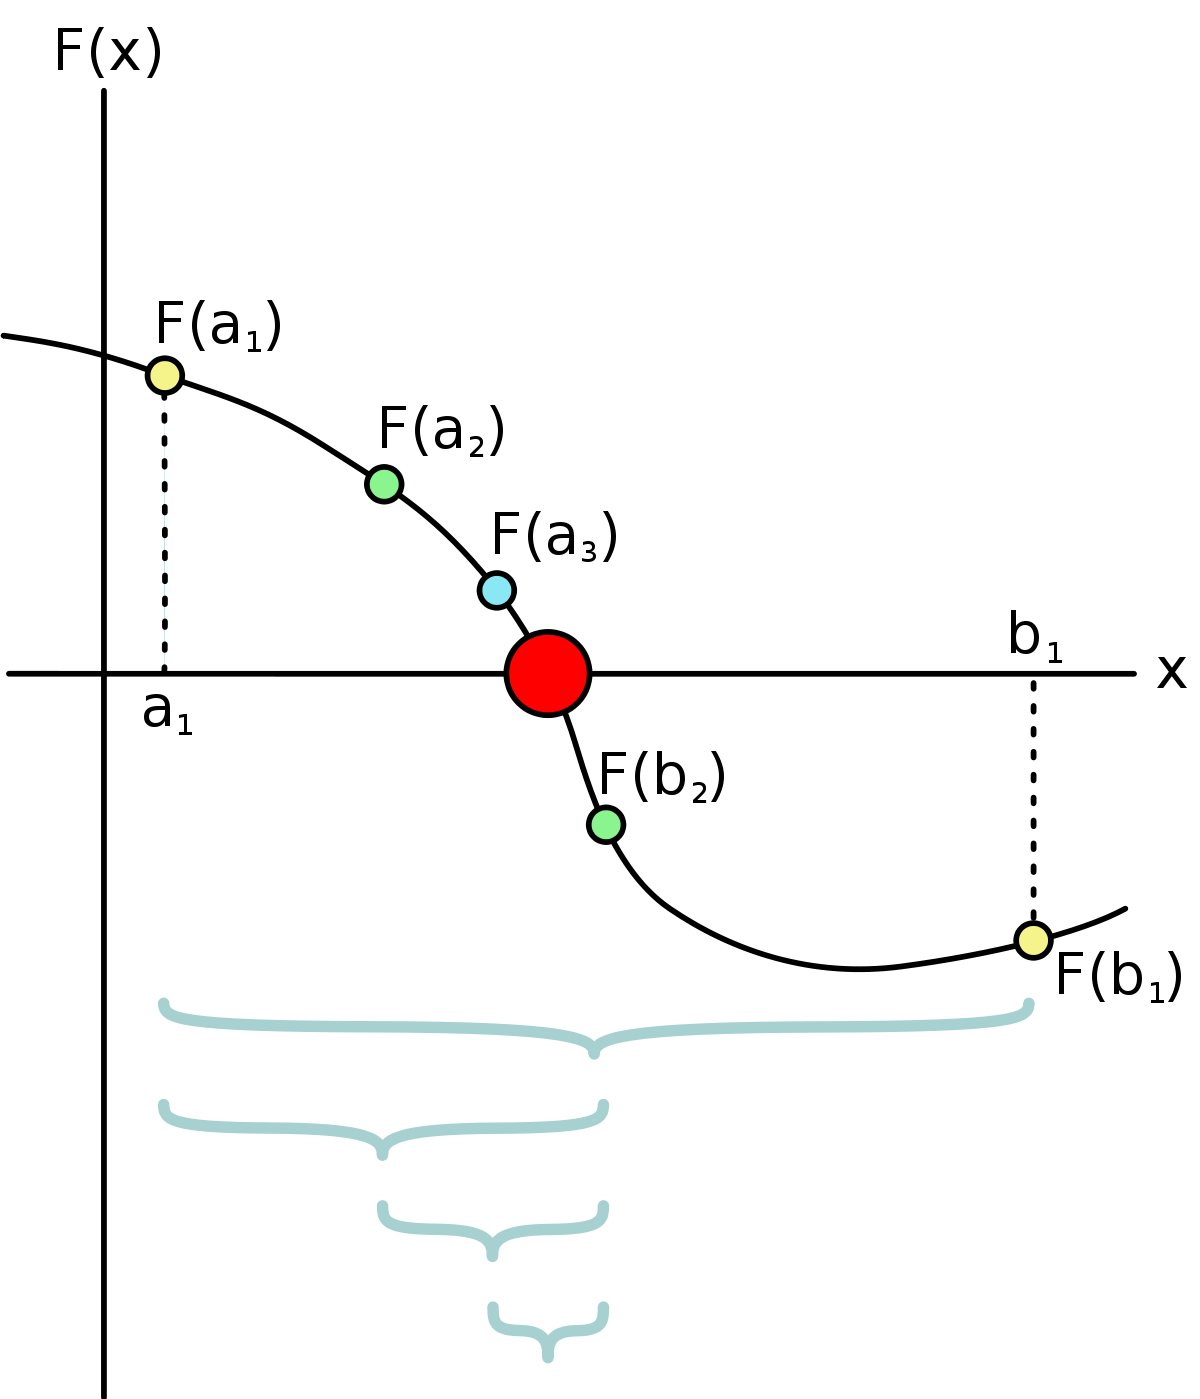
\includegraphics[scale=0.13]{biseccion.png}
\begin{observation}
	No hace falta que $f$ tenga una sola raíz en el intervalo.
	
	Uno va generando nuevos intervalos de la forma $[a_n,b_n]$ a la manera de búsqueda binaria. Asumamos que en ningún momento se choca con la raíz, porque ese caso no es interesante. Esto hace que $a_n$ sea creciente (y acotada superiormente por $b$) y $b_n$ decreciente (y acotada inferiormente por $a$). Luego $\exists lim a_n$ y $\exists lim b_n$. Y como $|b_n-a_n| \leq \frac{b-a}{2^n}\to 0$, se tiene que $lim a_n = lim b_n =: r$. (O sea, los intervalos son encajados y la longitud tiende a $0$ así que $\exists! r \in [a_n,b_n] \forall n$. Probemos que $f(r)=0$.\\
	
	En cada paso se verifica $f(a_n)f(b_) \leq 0$. Tomando límite, como $f$ es continua, obtenemos $f(r)^2 \leq 0$ entonces $f(r)=0$.
\end{observation}

\begin{lemma}
	Si definimos $x_x=\frac{a_{n-1}+b_{n-1}}{2}$ (es la sucesión que construimos para actualizar los intervalitos cambiando uno de los extremos por el punto medio), entonces tenemos:\\
	
	$|r-x_n|\leq \frac{1}{2}(b_{n-1}-a_{n-1})$. Basta separar en casos $r>x_n$ y $r<x_n$, deshacerse del módulo y acotar acordemente en cada caso.\\
	
	Pero sabemos que $\frac{1}{2}(b_{n-1}-a_{n-1}) = \frac{b-a}{2^n}$ luego hemos probado que $|r-x_n|\leq \frac{b-a}{2^n}$.
\end{lemma}

\subsection{Regula falsi}

Para este método, también llamado de falsa posición, vamos a pedir que haya una única raíz en el intervalo. \\

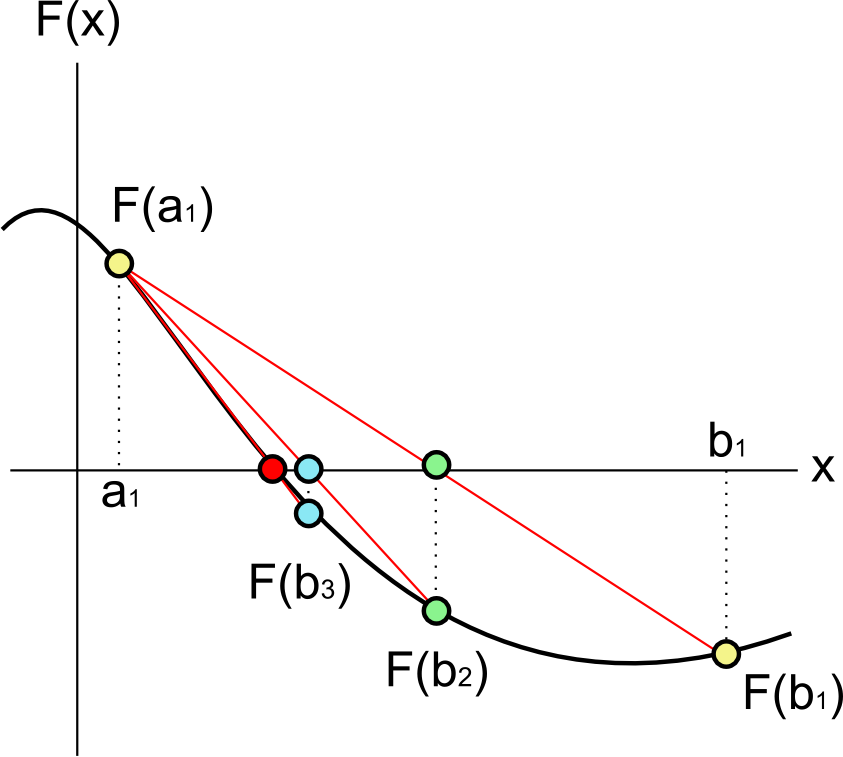
\includegraphics[scale=0.23]{regula_falsi.png}

Modificamos el método de bisección para en vez de tomar $x_n$ en la mitad del intervalo, tomarlo en la intersección de la recta secante $L$ y el eje $x$, donde $L$ une $f(a_n)$ con $f(b_n)$.

Podría suceder que la longitud de $I_n$ (los nuevos intervalos encajados) pero se tiene $x_n \to r$. ¿Por qué? ¿Vale siempre?

Probémoslo en el caso $x_n$ creciente, es decir, siempre reemplazamos $x_{n-1}$ por $x_n$ en los intervalos, con $x_0=a$.

El método entonces queda $x_{n+1} = x_n - \frac{f(x_n)}{f(b)-f(x_n)}(b-x_n)$

Tomando límite obtenemos $L = L - \frac{f(L)}{f(b)-f(L)}(b-L)$

De la igualdad anterior obtenemos $\frac{f(L)}{f(b)-f(L)}(b-L)=0$

SPG, supngamos $f(a)<0, f(b)>0$

Ahora bien, $f(x_n)<0 \forall n \Rightarrow f(L) \leq 0$. Esto quiere decir que $f(L) \neq f(b)$ y que en particular $L\neq b$. Luego puedo pasar las restas para el otro lado y queda $f(L) = 0$, como queríamos ver.


En la práctica, la hipótesis $x_n$ creciente no es tan brutal, porque con alguna hipótesis sobre $f''$ esto se obtiene. Por ejemplo, pidiendo $f C^2$ y $f''>0$ obtenemos que si $p_n(x)$ es la función lineal cuya raíz es $x_n$ entonces $p_n(x) \geq f(x)$. Luego, como $x_n$ cumple $p_n(x_n)=0$ entonces $f(x_n)\leq 0$. Si $f(x_n)=0$ para algún $n$ entonces ya ganamos, así que asumamos que no. Luego $f(x_n) < 0 \forall n$. Sucede algo análogo si $f''<0$.

Luego, si uno está en estas condiciones, puede asegurar teóricamente que el método converge. En la práctica suele funcionar bien incluso sin esta hipótesis.


\subsection{Newton-Raphson}

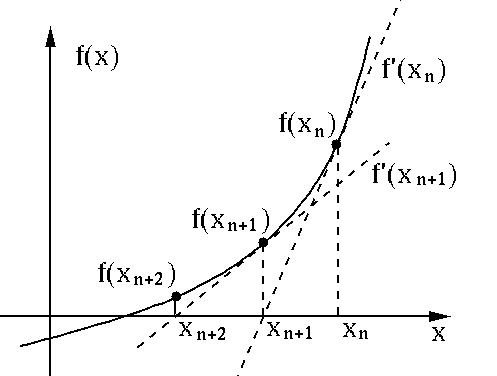
\includegraphics[scale=0.5]{newton_raphson.png}

La idea es construir el nuevo nodo a partir de la raíz de la recta tangente del nodo anterior.

Se toma $x_{n+1}$ tal que $f(x_n) + (x_{n+1}-x_n) f'(x_n) = 0$, o sea,
$x_{n+1} = x_n - \frac{f(x_n)}{f'(x_n)}$

Observar que debemos pedir $f$ derivable y $f' \neq 0$

\subsection*{Convergencia}

Asumamos que $r$ es una raíz simple de $f$, es decir, $f(r)=0, f'(r) \neq 0$ y supongamos $f''$ acotada.

Recordemos que definimos $e_n := x_n - r$ porque queremos que si estoy a la derecha el error sea positivo.

Tenemos $e_{n+1} = x_{n+1} - r = x_n - \frac{f(x_n)}{f'(x_n)} - r = e_n - \frac{f(x_n)}{f'(x_n)} = \frac{e_n f'(x_n)-f(x_n)}{f'(x_n)}$

El truco ahora es, para variar, hacer Taylor, pero centrado en $x_n$, y evaluar en $r$.

Tenemos $f(r) = 0 = f(x_n) + f'(x_n) (r-x_n) + \frac{f''(\xi) (r-x_n)^2}{2}= f(x_n) - f'(r) e_n + \frac{f''(\xi) e_n^2}{2}$.  Entonces $f'(r) e_n - f(x_n) = \frac{f''(\xi) e_n^2}{2}$

Peguemos las cosas. y juntando las cosas obtenemos $e_{n+1} = \frac{f''(\xi) e_n^2}{2 f'(x_n)}$.

Esto nos permite probar lo siguiente:

\begin{theorem}
Si $r$ es un cero simple de $f$ y $I=[r-\alpha,r+\alpha]$ es un intervalo tal que $|f'(x)|\geq \delta>0$ y $|f''(x)|\leq M$ en $I$ entonces:\\
$\exists \varepsilon > 0$ tal que $I_{\varepsilon} = [r - \varepsilon, r+\varepsilon] \subset I$ y se tiene que $|e_n| \to 0$ y $|e_{n+1}| \leq \frac{1}{2} \frac{M}{\delta} e_n^2$ siempre que $x_0 \in I_{\varepsilon}$.
\end{theorem}

\begin{proof}
	La cota sale de la discusión anterior. El $\varepsilon$ se construye aprovechando que aparece $e_n^2$ en la expresión. Sea $\varepsilon > 0$ tal que $frac{1}{2} \frac{M}{\delta} = \delta < 1$.
	 Luego $|e_0| = |x_0-r|\leq \varepsilon$, $|e_1| \leq \delta |e_0|$ y así siguiendo probamos $|e_n|\leq \delta^n |e_0| \to 0$.\\
	 Ojo: esta cota la tenemos que probar inductivamente, no podemos acotar directamente $e_n$ por $\delta$ ya que en principio no sabemos que $x_n$ queda dentro de $I_\varepsilon$.
\end{proof}

\begin{corollary}
	Si tenemos $f'$ continua, $f''$ acotada en $[a,b]$ y $r$ raíz simple de $f$ entonces como $f'(r)\neq 0$ por continuidad obtenemos que $\exists I \ni r$ tal que $f'\neq0$ en $I$ y caemos en las condiciones de arriba así que podemos asegurar convergencia.
\end{corollary}


\begin{definition}
	Decimos que un método es de orden $p$ si $\exists C > 0$ tal que $lim \frac{|e_{n+1}|}{|e_n|^p} = C$ y $\forall \varepsilon > 0$ vale que $lim \frac{|e_{n+1}|}{|e_n|^{p-\varepsilon}}=0$.
	
	Lo que está expresando esto es que $|e_{n+1}|\sim  C |e_n|^p$ 
\end{definition}

\begin{observation}
	Si converge, el método de NR es de orden 2 por la igualdad a la que llegamos al principio de la sección.
\end{observation}


\begin{theorem}
	Si $f$ es dos veces derivable y $f''>0$, es decir, $f$ es convexa, entonces el método de Newton-Raphson connverge $\forall x_0 \neq x^*$. Es decir, n este caso no hace falta pedir que $x_0$ esté cerca de $r$.
\end{theorem}

\begin{proof}

	Esta es la demostración del Durán:
	Podemos suponer que $f$ es monótona porque la iteración de Newton nunca irá a la izquierda.
	
	$Si x_0 > r$ entonces $r < x_1 < x_0$ y en general $x_0 > x_1 > ... > x_n > ... > r$. Luego la sucesión converge porque es monótona creciente y acotada superiormente. Haciendo álgebra de límites, si $\alpha$ es el límite, queda  $\alpha = \alpha - \frac{f(\alpha)}{f'(\alpha)}$ y como suponemos $f$ monótona $f'>0$.
	
	No estoy de acuerdo, porque suponer $f$ monótona es algo muy fuerte: supone que podemos cambiar $f$ por una función monótona derivable que la interpole en infinitos puntos. Es más, $f(x) = x^2$ no cumple $f'(\alpha) = f'(0) = 0$ así que la expresión no tiene sentido pero el algoritmo converge igual. 
\end{proof}

%TODO hacer punto fijo y método de la secante
\subsection{Punto fijo}
Los teoremas de existencia y unicidad de punto fijo salen.

\begin{theorem}
Sea $g :[a,b] \rightarrow \R\text{ tal que }|g(x)-g(y)|\leq k |x-y|\ \forall\ x,y\ \in [a,b]$ con $0<k<1$ y además $g([a,b]) \subset [a,b]$. \\

Entonces $g$ tiene un único punto fijo $r \in [a,b]$ y es límite de la sucesión

\begin{equation}
  \left\{
  \begin{array}{@{}ll@{}}
    x_0 \in [a,b] \text{ arbitrario} \\
    x_{n+1} = g(x_n)
  \end{array}\right.
\end{equation} 

Además, $\forall\ n$ se tiene $|x_n-r| \leq \frac{k^n}{1-k} |x_1-x_0|$ y también $|x_n-r|\leq k^n \underbrace{|x_0 -r|}_{\leq b-a}$ \\

Observación: La primera desigualdad nos permite acotar el error en función de algo fácilmente calculable.
\end{theorem} 

\begin{proof}
	Por las hipótesis se puede demostrar que existe un único punto fijo de $g$ al que llamaremos $r$.
	
	Tenemos $|e_{n+1}| = |x_{n+1} - r |= |g(x_n) - g(r)| \leq \lambda e_n  \leq ... \lambda^{n+1} e_0 \to 0$
	
	Es decir, tenemos $x_n \to r$.
	
	Por otra parte, tenemos $|x_0 - r| \leq |x_0 - x_1| + |x_1 - r| = |x_0 - x_1| + |g(x_0) - g(r)| \leq |x_0 - x_1| + \lambda |x_0 - r|$. Pasando $\lambda |x_0-r|$ para el otro lado obtenemos $|x_0-r| \leq (1-\lambda) |x_1-x_0|$. Luego $|e_n| \leq \lambda^n |x_0 - r| \leq \frac{\lambda}{1-\lambda} |x_1-x_0|$, como queríamos probar. 
\end{proof}


\begin{theorem}  Sea  $g :[a,b] \rightarrow \R$ es $C^1$ en $(a,b)$ y $r\in(a,b)$ un punto fijo de $g$. Si $|g'(r)|<1$ entonces $\exists\ \varepsilon>0$ tal que la iteración de antes es convergente siempre que $x_0 \in (r-\varepsilon,r+\varepsilon)$
\end{theorem} 

Observación: en la práctica vamos a probar que $g' < 1$ en un intervalito donde sabemos que hay un punto fijo porque no sabemos \textit{cuál} es el punto fijo.

\begin{proof}
	Como $|g'(r)|<1$, existe una constante $K<1$ y un $\varepsilon > 0$ tal que $|g'(x)|\leq K \forall x \in I_\varepsilon$, con $I_\varepsilon$ definido como antes. Esto vale por la continuidad de $g'$. Usando el TVM caemos en las condiciones de las hipótesis del teorema anterior.
\end{proof}

\subsection{Método de la secante}

Este método consiste en "ir por la secante" pero tomando los últimos dos nodos, en vez de Regula Falsi, que siempre tomaba un nodo y un extremo del intervalo. Observar que en este método no hay que tomar una decisión en base a un signo, a diferencia de Regula Falsi.

La recta que una $(x_{n-1},f(x_{n-1})$ con $(x_n,f(x_n)$ se puede construir con la forma de Lagrange o la de Newton. Usemos la de Newton, porque con ella va a quedar más clara la forma que tiene la iteración de este método (aunque, claro esa, con Lagrange también llegaríamos a lo mismo, pero había que sumar y restar cierto número y era más trabajo).

La recta es $y = f(x_n) + (x-x_n) \frac{f(x_n) - f(x_{n-1}}{x_n - x_{n-1}}$.

Igualando a cero obtenemos $x_{n+1} = x_n - f(x_n) \frac{x_n - x_{n-1}}{f(x_n) - f(x_{n-1}}$.

Observemos que la fración es un cociente incremental al revés, luego esta iteración es análoga a la de Newton Raphson $x_{n+1} = x_n - f(x_n) \cdot \frac{1}{f'(x_n)}$ pero cambiando la derivada por un cociente incremental.

Analicemos la convergencia, y el orden de convergencia de este método.

Sumando tenemos que $x_{n+1} = \frac{f(x_n) x_{n-1} - f(x_{n-1}}) x_n {f(x_n) - f(x_{n-1})}$, que de hecho es lo que habríamos obtenido si hubiéramos escrito la iteración a partir de la forma de Lagrange de la secante.

Luego $e_{n+1} = r - x_{n+1} = \frac{f(x_n) r- f(x_n) x_{n-1} - [f(x_{n-1} r - f(x_{n-1} x_n)]}{f(x_n) - f(x_{n-1})}$. Sacando factor común y reemplazando obtenemos:\\
$e_{n+1} = \frac{e_{n-1} f(x_n) - f(x_{n-1}) e_n}{f(x_n) - f(x_{n-1})}$\\

%TODO creo que hay un e_{n-1} mal
Ahora viene la parte divertida: quiero usar la magia de las diferencias divididas así que intercalo $f(r)$, que es $0$.\\

Obtengo $e_{n+1} = \frac{ e_{n-1} [f(x_n) - f(r)]- e_n [f(x_{n-1}) - f(r)] }{f(x_n) - f(x_{n-1})}$. Como quiero que aparezcan diferencias divididas, divido y multiplico por $e_n$ en el primer término del numerador y lo mismo con $e_{n-1}$ en el segundo término. Me queda lo siguiente:

$e_{n+1} = \frac{ -e_n e_{n-1} \frac{f(x_n) - f(r)}{x_n-r}+ e_n e_{n-1} \frac{f(x_{n-1}) - f(r)}{x_{n-1}-r} }{f(x_n) - f(x_{n-1})}$\\

\begin{caution}
Como $e_k = r - x_k$, los signos se dan vuelta.
\end{caution}

La cuenta, expresándola como diferencias, queda 

 $e_{n+1} = e_n e_{n-1} \frac{-f[r, x_n] + f[x_{n-1},r]}{f(x_n) - f(x_{n-1})}$, o, lo que es lo mismo:
 
 $e_{n+1} = - e_n e_{n-1} \frac{f[r, x_n] - f[x_{n-1},r]}{f(x_n) - f(x_{n-1})}$
 
 Multiplicando y dividiendo por $x_n - x_{n-1}$ obtenemos $e_{n+1} = - e_n e_{n-1} \frac{f[x_{n-1},r,x_n]}{f[x_{n-1},x_n]}$

Recordemos que queremos acotar esto. Vamos a necesitar el siguiente lema:

\begin{lemma}
	$f[a,b,c] = f''(\tau)$ 
\end{lemma}

\begin{proof}
	Tomo $g(x) = f(x) - \{f[a] + f[a,b] (x-a) + f[a,b,c] (x-a) (x-b) \}$ la resta entre $f$ y su polinomio interpolador en $a,b,c$.
	
	$g$ tiene 3 raíces (tal vez más). Luego $g'$ tiene al menos 2 raíces, y $g''$ tiene al menos 1. Pero $g''(x) = f''(x) - 2\cdot f[a,b,c]$. Si tomamos a $\tau$ como una raíz de $g''$ obtenemos lo deseado.
\end{proof}

Volviendo al error, obtenemos entonces que $\exists\ \tau_n$ tal que $e_{n+1} = -\frac{1}{2}
\frac{f''(\tau_n)}{f'(\chi_n)} e_n e_{n-1}$, donde para el denominador usamos simplemente TVM.


\begin{theorem}
	Si $f'(r) \neq 0, ||f''|\leq K$ en un entorno de $r$ y $x_0,x_1$ están suficientemente cerca de $r$ entonces $e_n \to 0$.
\end{theorem}

\begin{proof}
	Como $f'(r) \neq 0, \exists\ \varepsilon>0$ tal que $f' \geq \delta$ en $I_\varepsilon$. Achiquemos $\varepsilon$ para que $|f''| \geq K$ allí. Luego si $x_0,x_1 \in I_\varepsilon$ entonces $|e_2| \leq \frac{K}{2 \delta} |e_1| |e_0| \leq \frac{K}{2 \delta} \varepsilon^2$. Podemos achicar $\varepsilon$ aun más para que $\frac{K}{2 \delta} \varepsilon = \delta < 1$. Luego obtenemos que $x_2 \in I_\varepsilon$.\\

Inductivamente se prueba que $e_n \leq \delta^{n-1} \varepsilon \to 0$.
\end{proof}

Estudiemos el orden de convergencia del método en las condiciones anteriores (del teorema).

Sea $c_n =  \frac{f''(\tau_n)}{f'(\chi_n)}$. Con un argumento de continuidad, si tenemos que $e_n \to 0$ entonces $c_n \to c_\infty = \frac{f''(r)}{f'(r)}$ y asumamos $f''(r) \neq 0$ así $c_\infty \neq 0$. \bigskip

Buscamos $p$ tal que $\underset{n\to 0}{lim}\ \frac{|e_{n+1}|}{|e_n|^p}=C \neq 0$.

Tenemos $\frac{|e_{n+1}|}{|e_n|^p} = |c_n| |e_n|^{1-p} |e_{n-1}|$ (ojo, no sirve reemplazar $e_n$ por lo que es).

Quiero expresar esto como una iteración de punto fijo para alguna elección de $p$ para que esto converja. Quiero que la sucesión sea $y_n = \frac{|e_{n+1}|}{|e_n|^p}$. Luego llevo la parte de la derecha a que tenga esa forma, con $e_n$ arriba y $e_{n-1}$ abajo:


%TODO arreglar estos parentesis horribles


$|c_n| |e_n|^{1-p} |e_{n-1}| = |c_n| (\frac{|e_n|}{|e_{n-1}^p})^\alpha$, para algún $\alpha$ acorde. Se ve que $\alpha$ debe cumplir $\alpha = 1-p$ y $\alpha\cdot p = -1$.

Luego tenemos $p\cdot\alpha = p - p^2 = -1$. Como necesitamos $p>0$ al hacer la resolvente nos quedamos con la raíz $p=\frac{1+\sqrt{5}}{2}$.

Si definimos $y_n$ como antes, obtenemos que $y_{n+1} = c_n y_n^{\frac{-1}{p}}$. Como $p>1$ se puede ver que la iteración converge.% a $x$ donde $x = c_\infty x^{\frac{-1}{p}}$, es decir, $x=c\_infty^{\frac{1}{p}}$.

%TODO se llamaban lineales?
\section{Métodos multipaso lineales}

\section{Cosas que me falta entender bien}
\begin{itemize}
	\item El método iterativo del gradiente
	\item La desigualdad difícil del teorema del número de condición y matrices singulares, aunque no creo que lo tomen.
	\item Consistencia + Estabilidad $\Rightarrow$ convergencia (y qué es cada cosa y cómo hacer cuentas, por el amor de dios)
	\item Todo el tema de resolución de ecuaciones no lineales
	\item Métodos multipaso
\end{itemize}



\section{Algunos supuestos errores que encontré en el Durán-Lasalle-Rossi}

\begin{itemize}
	\item En la expresión (4.7) de la página 81 (método de la secante), donde se define $g(x)$, falta un paréntesis. Debería ser:
$g(x) = f(x) - \Bigg((f(a) + f[a,b] (x-a) + f[a,b,c] (x-a) (x-b))\Bigg)$ ya que definimos a la función para que en $a,b,$ y $c$ de $0$.
	\item La figura 4.3 de la página 70 (método de Newton-Raphson) está mal. Observar que desde $x_0$ se está yendo por la tangente hasta intersecar el gráfico de la función y no el eje $x$.
	\item En la demostración del teorema 4.11 de la página 76 (método de Newton-Raphson), se asume que $f$ es monótona porque de todas maneras la iteración de Newton nunca irá a la izquierda. Esto no lo señalo como error, pero no estoy de acuerdo con la asumpción. En primer lugar, la función $f(x) = x^2$ es convexa pero no monótona. El algoritmo converge pero $f'(r) = f'(0) = 0$. Me pregunté si lo que se insinuaba era que podían cambiar la función $f$ por otra que sea monótona que la interpole en los puntos $x_i$ pero sabemos interpolar finitos puntos, no infinitos. Update: revisé la cursada de este cuatrimestre y mencionan que $f(x) = x^2-4$ cumple que si empezás en $x_0=0$, como $f'(0)=0$, el algoritmo no anda.
	 \item En la página 83, al final de la demostración del orden de convergencia del método de la secante sea afirma que el punto fijo es $\hat{x} = c_\infty^\frac{1}{p}$. Pero al reemplazar en la ecuación no da. No sé si esto es un error igual, tal vez estoy entendiendo mal. A mí me da distinto, pero lo importante es que da un número.
	\item En la página 71 el error de Newton Raphson se define como $e_{n+1} = x_{n+1} -r$, pero para el método de la secante se define al revés, $e_{n+1} = r - x_{n+1}$. No es realmente un error, uno lo define como quiere, pero puede confundir a la hora de hacer cuentas (¿si uno prueba que el error es positivo lo intuitivo no sería que la sucesión esté a la derecha de la raíz?)
	\item En la página 174, en el ejemplo 8.5, hay un error de tipeo. Donde dice "para aproximar $\sqrt{2}$ debería decir "para aproximar $\sqrt{t}$" (es solución de la ecuación).
\end{itemize}


\section{Ejercicios de final}

\subsection{Ejercicio 2 Examen final 19/3/04}

i) Demostrar que el método de Gauss-Seidel converge para matrices de diagonal estrictamente dominante.

ii) Dada la matriz
%TODO no se hacer matrices

$$a\ c\ 0$$
$$c\ a\ c$$
$$0\ c\ a$$\\

dar condiciones necesarias y suficientes sobre $a,c\in \mathbb{R}$ para la convergencia de los métodos de Jacobi y Gauss-Seidel aplicados a la resolución de $Ax=b$.

Resolución:

i) Hecho en la parte de teoría.\\

ii) Ambos métodos convergen si y solo si $\rho(A)<1$.


\iffalse
Calculemos el determinante de  :

$$(a - \lambda)\ c\ 0$$
$$c\ (a-\lambda)\ c$$
$$0\ c\ (a-\lambda)$$\\

para obtener los autovalores.

Obtenemos $(a-\lambda) [(a-\lambda)^2 - c^2] - c [c (a-\lambda) - c \cdot 0]$. Desarrollar esta expresión haciendo distributivas no sería muy efectivo.\\

Es mejor observar que la expresión queda $(a-\lambda)^3 - (a-\lambda) c^2 - c^2 (a-\lambda) = (a-\lambda)^3 - 2(a-\lambda) c^2 = (a-\lambda) [(a-\lambda)^2 - 2c^2)]$.\\

Si igualamos a $0$ (porque estamos buscando las raíces) obtenemos que $\lambda = a$ ó $(a-\lambda)^2 = 2c^2)$

Luego obtenemos la condición necesaria $|a|<1$ (en el caso $\lambda = a$.

Trabajemos el otro caso: $(a-\lambda)^2 = 2c^2) \Leftrightarrow a - \lambda = \sqrt{2}|c| \Leftrightarrow \lambda = a - \sqrt{2} |c|$

Obtenemos la condición necesaria $|a-\sqrt{2} |c|\ | <1$ y juntando ambas condiciones obtenemos $\rho(A) < 1$. Pero la segunda condición se puede trabajar un poco más.\\

Observemos que ya es condición necesaria $|a|<1 \Rightarrow -1 < a < 1$

%Además $a-\sqrt{2} |c|<1$. Juntando queda $-1 -\sqrt{2} |c|< a -\sqrt{2} |c| < a-\sqrt{2} |c| < 1$. Mirando los extremos de la cadena de desigualdades obtenemos $-\sqrt

%$-1 < a-\sqrt{2} |c| < 1 - \sqrt{2} |c| \Rightarrow \sqrt{2} |c| < 2 \Rightarrow |c| < \sqrt{2}$

La condición $a-\sqrt{2} |c| < 1$ se cumple directamente ya que $a<1$ y $\sqrt{2} |c|>0$.

$a - \sqrt{2}|c| > -1 \Leftrightarrow a > -2 + \sqrt{2} |c| \Leftrightarrow |c| < \frac{a+1}{\sqrt{2}}$

Luego las condiciones necesarias y suficientes son $|a|<1, |c| < \frac{a+1}{\sqrt{2}}$

\fi


Como es tridiagonal basta que lo veamos para Jacobi.

Analizando el determinante de $B_J = - D^{-1} (L+U)$, obtenemos que los autovalores son $0$ y $\pm \sqrt{2} \frac{|c|}{|a|}$. Luego como necesitamos $\rho(B_J) < 1$ pedimos $|c|<\frac{|a|}{\sqrt{2}}$ y estamos.

(Es más fácil analizar los autovalores de la matriz con el truquito $\lambda$ autovalor de $B = -M^{-1} N \Leftrightarrow det(M\lambda + N) = 0$

\subsection{Ejercicio 1 Examen final 16/6/04}
Ejercicio 1.

%TODO no se por qué no anda \R acá
i) Dada $f:[a,b] \rightarrow \mathbb{R}$, dar condiciones sobre $f$ que garanticen que la sucesión dada por la iteración $x_{n+1} = f(x_n)$ converge a un punto fijo de $f$. Demostrarlo.\\

ii) ¿Cuál es el valor de la siguiente expresión?

$L = \sqrt{2 + \sqrt{2 + \sqrt{2+...}}}$


Resolución:

i) Es un teorema. \\

ii) La igualdad de arriba se puede expresar como el límite de una sucesión:

$x_0 = \sqrt{2}$\\
$x_1 = \sqrt{2 + \sqrt{2}}$\\
$x_2 = \sqrt{2 + \sqrt{2 + \sqrt{2}}}$
y así siguiendo.

Luego tenemos que si definimos $f(x) = \sqrt{2 + x}$, y $x_0 = 0$, $x_{n+1} = f(x_n) \Rightarrow L = lim\ x_n$.

Dos observaciones: En primer lugar, hay que chequear que efectivamente la sucesión sea convergente. En segundo lugar, cualquier otro $x_0$ también servía.

Tenemos que $f'(x) = \frac{1}{2 \sqrt{2+x}}$

Es puras cuentas ver que $|f'(x)|<1 - \varepsilon \Leftrightarrow x > \frac{-7}{4} - \hat{varepsilon}$ para cierto $\hat{varepsilon}$.

Lo que dice esta cuenta es que el intervalo donde vamos a trabajar tiene que empezar necesariamente a la derecha de $\frac{-7}{4}$. Pero...¿dónde termina?\\

Observemos que $f'\geq 0$. Luego, si la sucesión converge, necesariamente convergerá crecientemente al punto fijo. Entonces necesitaremos probar que la sucesión siempre queda a la izquierda del punto fijo.\\

Finjamos que ya tenemos el intervalo y sabemos que la sucesión converge. Entonces tenemos $L = \sqrt{2 + L}$. Luego $L^2 - 2 - L = 0 \Rightarrow L=2$ ó $-1$. Pero $L\geq 0$ porque $x_n \geq 0\ \forall\ n$. Luego $L=2$.\\

Esto nos sugiere, entonces, trabajar con $I = [a,2]$ con $a > \frac{-7}{4}$. Tomemos $a=0$.\\

Veamos que $f(I) \subset I$. Como $f$ es creciente, basta ver que si $x<2 \Rightarrow f(x) < 2$, pero esto es cierto porque $\sqrt{2+x}<2 \Leftrightarrow 2 +x<4 \Leftrightarrow x < 2$. Luego como en $I$ $f' \leq \delta < 1$ para cierto $\delta$ y $f(I) \subset I$, tenemos que la sucesión efectivamente converge y entonces $L=2$.

%TODO hacer la demo del método de la secante

\subsection{Ejercicio 3 Examen final 19/03/04}

Sea $f(x) 0 \frac{x}{1+|x|}$. Determinar para qué valores de $x_0$ la iteración dada por el método de Newton-Raphson es convergente, para cuáles es divergente, y cuándo se obtienen ciclos periódicos.

Resolución: es fácil chequear que $0$ es la única raíz de $f$. Si hice bien las cuentas, $f'(x) = \frac{1}{(1+|x|)^2}$. Luego la iteración de Newton Raphson es $x_{n+1}=x_n - \frac{f(x_n)}{f'(x_n)} = x_m - \frac{x_n}{1+|x_n|} \cdot (1+|x_n|)^2  \underset{simplifico}{=} x_n - x_n (1+|x_n|) = x_n - x_n + x_n |x_n| = x_n |x_n|$

Como $r=0$, $|e_{n+1}| = |x_n|^2 \to 0 \Leftrightarrow |x_0| < 1$. Se puede ver que si $|x_0|=1$ obtengo ciclos periódicos.

\begin{caution}
	En este caso analizar el error con la fórmula con la derivada segunda no me sirvió de mucho (no llegué a nada útil)
\end{caution}



\subsection{Ejercicio 21 práctica 7}

Sea $f \in C^2[a,b]$, y sean $x_0 = a, x_1 = a + h,...,x:n=b$. Considerar la poligonal $\ell(x)$ que interpola a $f$ en los puntos $x_i$.

a) Probar que $|f(x)-\ell(x)| \leq \frac{h^2}{2} max |f''(x)|$\\

Resolución: es estándar. \bigskip

b) Para los $x$ donde $\ell$ es derivable, probar que $|f'(x)-\ell'(x)| \leq h\ max |f''(x)|$\\

Resolución: $\ell$ es derivable adentro de cada subintervalo. Si es derivable en un extremo de un subintervalo, entonces las pendientes de $\ell$ en el subintervalo a izquierda y el subintervalo a derecha son iguales y puedo considerar que es un solo subintervalo y mirar al punto donde es derivable como parte de un abierto donde la función es derivable.\\

La observación clave es que $g(x) = f(x) - \ell(x)$ tiene al menos dos raíces en cada subintervalo cerrado. Luego $g'(x) = f'(x) - \ell'(x)$ tiene al menos una raíz, por Rolle. Es decir, obtuvimos que $\ell'$ interpola a $f'$ al menos una vez en cada subintervalo, lo cuál es bastante increíble porque estamos hablando de la derivada de una poligonal, que es constante. Luego podemos usar la cota estándar para polinomios interpoladores de grado cero, y así obtenemos lo deseado.

\end{document}